\documentclass[aspectratio=169]{beamer}

\usepackage{amsmath, amssymb, amsxtra, amsthm, amsfonts}
\usetheme{moloch}
\usecolortheme{beaver}
\setbeamertemplate{footline}
{
  \leavevmode%
  \hbox{%
    \begin{beamercolorbox}[wd=.5\paperwidth,ht=2.25ex,dp=1ex,center]{author in head/foot}%
      \usebeamerfont{author in head/foot}\insertsection
    \end{beamercolorbox}%
    \begin{beamercolorbox}[wd=.5\paperwidth,ht=2.25ex,dp=1ex,right]{date in head/foot}%
      \usebeamerfont{date in head/foot}\inserttitle\hspace*{2em}
      \insertframenumber{} / \inserttotalframenumber\hspace*{2ex}
    \end{beamercolorbox}}%
  \vskip0pt%
}
\makeatother

\usepackage[english]{babel}
\usefonttheme{serif}

\usepackage{mathtools}
\usepackage{graphicx}
\usepackage{bm}
\usepackage{color}
\usepackage[dvipsnames,table]{xcolor}
\usepackage{tikz}
\usepackage{stanli}
\usepackage{verbatim}
\usepackage{tikz}
\usetikzlibrary{shapes,calc,through,3d,patterns}
\usetikzlibrary{decorations.pathreplacing}
\usetikzlibrary{arrows.meta,calc,positioning}

\usepackage{pgfplots}
\usepackage{siunitx} % For formatting numbers
\usepackage{hyperref}
\hypersetup{colorlinks=true,linkcolor=darkred}
\usepackage{multicol}
\usepackage[absolute,overlay,]{textpos}
\usepackage{pgfplots}
\pgfplotsset{width=10cm,compat=1.9}
\usepackage{subcaption}
\usepackage{multirow}
\usepackage{bbding}
\usepackage{arydshln}
\usepackage{mathtools}
\usepackage{tcolorbox}
\usepackage{animate}

\textblockorigin{80mm}{45mm}


\newtheorem{thm}{Theorem}
\newtheorem{cor}[thm]{Corollary}
\newtheorem{prop}[thm]{Proposition}
\newtheorem{lem}[thm]{Lemma}
\theoremstyle{remark}
\newtheorem*{rem}{Remark}

%Block def
\definecolor{darkred}{rgb}{0.6,0,0}
\setbeamertemplate{blocks}[rounded][shadow=false]
\setbeamercolor{block title}{bg=darkred!15,fg=black}
\setbeamercolor{block body}{bg=darkred!5,fg=black}

\setbeamercolor{itemize item}{fg=darkred}
\setbeamercolor{itemize subitem}{fg=darkred}
\setbeamercolor{itemize subsubitem}{fg=darkred}
\setbeamercolor{enumerate item}{fg=darkred}
\setbeamercolor{button}{bg=gray!30,fg=darkred}

\setbeamertemplate{itemize item}[square]
\setbeamertemplate{itemize subitem}[circle]
\setbeamertemplate{itemize subsubitem}[triangle]
\setbeamertemplate{enumerate items}[circle]
\setbeamercolor{item projected}{bg=darkred}

\newcommand{\bolddelta}{\boldsymbol\delta}
\newcommand{\boldxi}{\boldsymbol\xi}
\DeclareMathOperator*{\A}{\text{\raisebox{-0.2cm}{\Huge A}}}




\title{Finite element method}
\subtitle{Linear elastodynamics}
\author{ME473 Dynamic finite element analysis of structures}
\institute{Stefano Burzio}
\date{2025}

\begin{document}
\usenavigationsymbolstemplate{}
{\setbeamertemplate{footline}{}

    \frame{\titlepage
        \begin{tikzpicture}[overlay, remember picture]
            \node[anchor=north east, xshift=-.9cm] at (current page.north east) {
\includegraphics[width=2cm]{../images/epfl_logo.png}};
            \node[anchor=south east, xshift=-.87cm, yshift=.05cm] at (current page.south east)  {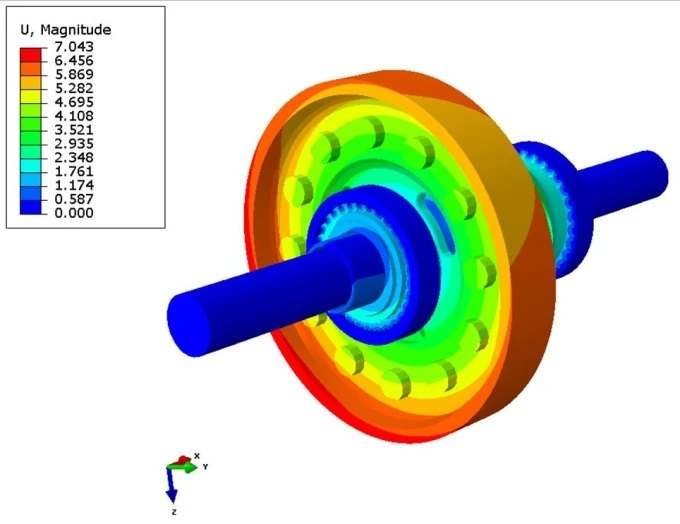
\includegraphics[width=5cm]{../images/dynamic-analysis.jpg}};
        \end{tikzpicture}
    }

    \begin{frame}{Where do we stand?}
        \begin{center}
            \begin{tabular}{|c|l|l|l|}
                \hline
                \rowcolor{darkred!20}\textbf{Week} & \textbf{Module}                          & \textbf{Lecture topic}             & \textbf{Mini-projects} \\
                \hline
                1                                  & \multirow{5}{7em}{Linear elastodynamics} & Strong and weak forms              &                        \\ \cline{1-1} \cline{3-4}
                2                                  &                                          & Galerkin and FE methods            &                        \\ \cline{1-1} \cline{3-4}
                3                                  &                                          & Systematisation of the procedure   & Groups formation       \\ \cline{1-1} \cline{3-4}
                4                                  &                                          & 3d elements, numerical integration & Project 1 statement    \\
                \cline{1-1} \cline{3-4}
                \hline
            \end{tabular}
        \end{center}
        \vspace{1cm}
    \end{frame}

    \begin{frame}
        \textbf{\large Summary}
        \begin{itemize}
            \item Recap week 3
            \item Solid finite elements
            \item Numerical integration
            \item Examples
                  \begin{itemize}
                      \item MATLAB PDE Toolbox
                      \item Ansys
                      \item Abaqus
                            end{itemize}
                  \end{itemize}
        \end{itemize}

        \vspace{.5cm}

        \textbf{\large Recommended readings}
        \begin{enumerate}
            \item Gmür, Dynamique des structures (§3.1, §3.2, and §3.3)
        \end{enumerate}
    \end{frame}
}

\section{Recap week 3 \\ Finite element method local approach}
 {\setbeamercolor{background canvas}{bg=darkred!5}
  \setbeamercolor{block body}{bg=darkred!5,fg=black}


  \begin{frame}{Localization and assembly}
      \begin{itemize}
          \item \textbf{Localization:} real and virtual displacements are restricted to each finite element and are expressed in terms of local shape functions and nodal displacements:
                $$
                    {}^e\mathbf{u}^h(\mathbf{x}, t) = {}^e\mathbf{H}(\mathbf{x}) {}^e\mathbf{q}(t) \quad\text{and}\quad {}^e\bolddelta \mathbf{u}^h(\mathbf{x}) = {}^e\mathbf{H}(\mathbf{x}) ^e\bolddelta\mathbf{q}.
                $$
          \item \textbf{Localization matrices \( {}^e\mathbf{L} \) :} boolean matrices that map local to global node numbering.
          \item \textbf{Elementary quantities:} elementary stiffness matrix \( {}^e\mathbf{K} \), elementary mass matrix \( {}^e\mathbf{M} \), and elementary force vector \( {}^e\mathbf{r} \) are computed for each element.

          \item \textbf{Assembly:} global matrices and vectors are assembled using the localization matrices:
                \[
                    \mathbf K =\A_{e=1}^m {}^e\mathbf K = \sum_{e=1}^{m} {}^e\mathbf L^T {}^e\mathbf K{}^e\mathbf L \quad\text{and}\quad  \mathbf r =\A_{e=1}^m {}^e\mathbf r = \sum_{e=1}^{m} {}^e\mathbf L^T {}^e\mathbf r
                \]
      \end{itemize}
  \end{frame}

  \begin{frame}{The local finite element point of view (in 2d)}
      \vspace{-1cm}
      \begin{columns}[T]
          \begin{column}{.4\textwidth}
              \begin{center}
                  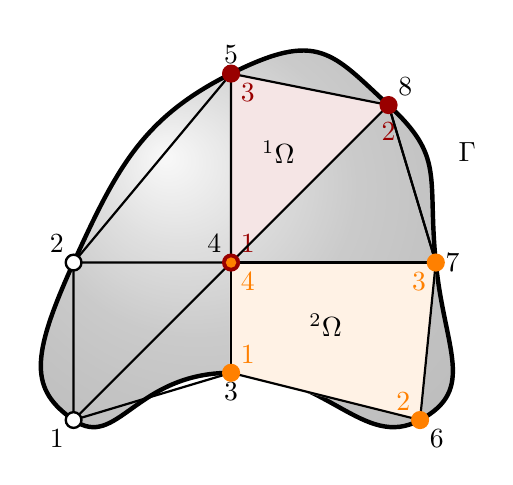
\begin{tikzpicture}[scale=2]
                      % \draw[step=1.0,black,thin] (0,0) grid (4,4);
                      % Draw the potato-like shape
                      \shade [ball color= gray!90!black, opacity=.3] plot [thick,smooth cycle, tension=1] coordinates  {(1,2) (2,3.2) (3,3) (3.3,2) (3.2,1) (2,1.3) (1,1)};
                      \draw[ultra thick] plot [thick,smooth cycle, tension=1] coordinates {(1,2) (2,3.2) (3,3) (3.3,2) (3.2,1) (2,1.3) (1,1)};
                      \draw[fill=darkred!30,thick,darkred!10] (2,2) -- (3,3) -- (2,3.2) -- cycle;
                      \draw[fill=orange!30,thick,orange!10] (2,2) -- (3.3,2) -- (3.2,1) -- (2,1.3) -- cycle;
                      % label the nodes
                      \node[below left] at (1,1) {$1$};
                      \node[above left] at (1,2) {$2$};
                      \node[below] at (2,1.3) {$3$};
                      \node[orange,above right] at (2,1.3) {$1$};
                      \node[above left] at (2,2) {$4$};
                      \node[darkred,above right] at (2,2) {$1$};
                      \node[orange,below right] at (2,2) {$4$};
                      \node[above] at (2,3.2) {$5$};
                      \node[darkred,below right] at (2,3.2) {$3$};
                      \node[below right] at (3.2,1) {$6$};
                      \node[orange,above left] at (3.2,1) {$2$};
                      \node[right] at (3.3,2) {$7$};
                      \node[orange,below left] at (3.3,2) {$3$};
                      \node[above right] at (3,3) {$8$};
                      \node[darkred,below={3pt}] at (3,3) {$2$};
                      % Label the region Omega
                      \node at (2.3,2.7) {${}^1\Omega$};
                      \node at (2.6,1.6) {${}^2\Omega$};
                      % Label the boundary Gamma
                      \node at (3.5,2.7) {$\Gamma$};
                      \draw[thick] (1,2) -- (2,3.2) -- (3,3) -- (3.3,2) -- (3.2,1) -- (2,1.3) -- (1,1) -- cycle;
                      \draw[thick] (1,2) -- (2,2) -- (3,3) -- (3.3,2);
                      \draw[thick] (2,1.3) -- (2,2) -- (3.3,2);
                      \draw[thick] (1,1) -- (2,2) -- (2,2.3) -- (2,3.2);
                      \node[darkred,draw,shape=circle,fill=darkred,minimum size=2mm,line width=0.3mm,inner sep=0] at (2,2) {};
                      \node[orange,draw,shape=circle,fill=orange,minimum size=1mm,line width=0.3mm,inner sep=0] at (2,2) {};
                      \node[draw,shape=circle,fill=white,minimum size=2mm,line width=0.3mm,inner sep=0] at (1,1) {};
                      \node[draw,shape=circle,fill=white,minimum size=2mm,line width=0.3mm,inner sep=0] at (1,2) {};
                      \node[orange,draw,shape=circle,fill=orange,minimum size=2mm,line width=0.3mm,inner sep=0] at (2,1.3) {};
                      \node[darkred,draw,shape=circle,fill=darkred,minimum size=2mm,line width=0.3mm,inner sep=0] at (2,3.2) {};
                      \node[darkred,draw,shape=circle,fill=darkred,minimum size=2mm,line width=0.3mm,inner sep=0] at (3,3) {};
                      \node[orange,draw,shape=circle,fill=orange,minimum size=2mm,line width=0.3mm,inner sep=0] at (3.2,1) {};
                      \node[orange,draw,shape=circle,fill=orange,minimum size=2mm,line width=0.3mm,inner sep=0] at (3.3,2) {};
                  \end{tikzpicture}
              \end{center}
          \end{column}
          \begin{column}{.6\textwidth}
              Every finite element ${}^e\Omega$ has:
              \begin{itemize}
                  \item Number of nodes ${}^ep$,
                  \item Connectivity $({}^ep\times 1)$,\vspace{5pt}
                  \item ${}^e\mathbf{q}$ vector of nodal displacements ($2{}^e p\times 1$),
                  \item ${}^e\mathbf{u}$ vector of displacements ($2\times 1$), \vspace{5pt}
                  \item ${}^eh_i$ local shape functions  ($i=1,\dots, {}^ep$),
                  \item $^e\mathbf{H}$ local shape functions matrix ($2\times 2{}^e p$), \vspace{5pt}
                  \item $^e\mathbf{K}$ local stiffness matrix ($2{}^e p\times 2{}^e p$),
                  \item $^e\mathbf{M}$ local mass matrices ($2{}^e p\times2{}^e p$),
                  \item $^e\mathbf{r}$ local loads vector ($2{}^e p\times 1$).
              \end{itemize}
          \end{column}
      \end{columns}
  \end{frame}

  \begin{frame}{Archetypal to local}
      \begin{center}
          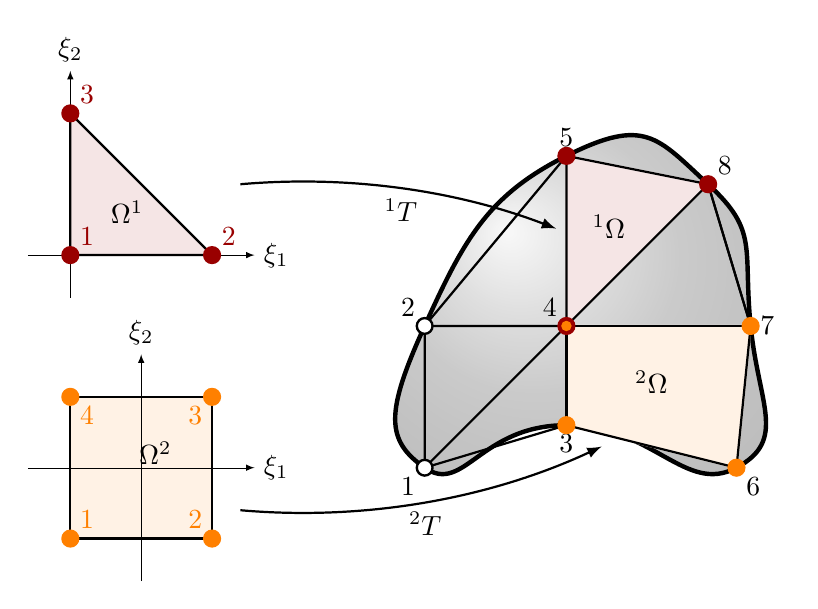
\begin{tikzpicture}[scale=1.8]
              % \draw[step=1.0,black,thin] (-2,0) grid (4,4);
              % Draw the potato-like shape
              \shade [ball color= gray!90!black, opacity=.3] plot [thick,smooth cycle, tension=1] coordinates  {(1,2) (2,3.2) (3,3) (3.3,2) (3.2,1) (2,1.3) (1,1)};
              \draw[ultra thick] plot [thick,smooth cycle, tension=1] coordinates {(1,2) (2,3.2) (3,3) (3.3,2) (3.2,1) (2,1.3) (1,1)};
              \draw[fill=darkred!30,thick,darkred!10] (2,2) -- (3,3) -- (2,3.2) -- cycle;
              \draw[fill=orange!30,thick,orange!10] (2,2) -- (3.3,2) -- (3.2,1) -- (2,1.3) -- cycle;
              % label the nodes
              \node[below left] at (1,1) {$1$};
              \node[above left] at (1,2) {$2$};
              \node[below] at (2,1.3) {$3$};
              \node[above left] at (2,2) {$4$};
              \node[above] at (2,3.2) {$5$};
              \node[below right] at (3.2,1) {$6$};
              \node[right] at (3.3,2) {$7$};
              \node[above right] at (3,3) {$8$};
              % Label the region Omega
              \node at (2.3,2.7) {${}^1\Omega$};
              \node at (2.6,1.6) {${}^2\Omega$};
              \draw[thick] (1,2) -- (2,3.2) -- (3,3) -- (3.3,2) -- (3.2,1) -- (2,1.3) -- (1,1) -- cycle;
              \draw[thick] (1,2) -- (2,2) -- (3,3) -- (3.3,2);
              \draw[thick] (2,1.3) -- (2,2) -- (3.3,2);
              \draw[thick] (1,1) -- (2,2) -- (2,2.3) -- (2,3.2);
              \node[darkred,draw,shape=circle,fill=darkred,minimum size=2mm,line width=0.3mm,inner sep=0] at (2,2) {};
              \node[orange,draw,shape=circle,fill=orange,minimum size=1mm,line width=0.3mm,inner sep=0] at (2,2) {};
              \node[draw,shape=circle,fill=white,minimum size=2mm,line width=0.3mm,inner sep=0] at (1,1) {};
              \node[draw,shape=circle,fill=white,minimum size=2mm,line width=0.3mm,inner sep=0] at (1,2) {};
              \node[orange,draw,shape=circle,fill=orange,minimum size=2mm,line width=0.3mm,inner sep=0] at (2,1.3) {};
              \node[darkred,draw,shape=circle,fill=darkred,minimum size=2mm,line width=0.3mm,inner sep=0] at (2,3.2) {};
              \node[darkred,draw,shape=circle,fill=darkred,minimum size=2mm,line width=0.3mm,inner sep=0] at (3,3) {};
              \node[orange,draw,shape=circle,fill=orange,minimum size=2mm,line width=0.3mm,inner sep=0] at (3.2,1) {};
              \node[orange,draw,shape=circle,fill=orange,minimum size=2mm,line width=0.3mm,inner sep=0] at (3.3,2) {};
              % Draw master square
              \draw[fill=orange!30,thick,orange!10] (-1.5,0.5) -- (-0.5,0.5) -- (-0.5,1.5) -- (-1.5,1.5) -- cycle;
              \draw[thick] (-1.5,0.5) -- (-0.5,0.5) -- (-0.5,1.5) -- (-1.5,1.5) -- cycle;
              \draw[ultra thin,-latex] (-1.8,1) -- (-0.2,1) node[right]{$\xi_1$};
              \draw[ultra thin,-latex] (-1,0.2) -- (-1,1.8) node[above]{$\xi_2$};
              \node at (-0.9,1.1) {$\Omega^2$};
              \draw[thick,-latex] (-0.3,0.7) arc [start angle=-95, end angle=-65, radius=5] node[midway, below]{${}^2T$};
              \node[orange,draw,shape=circle,fill=orange,minimum size=2mm,line width=0.3mm,inner sep=0] at (-1.5,0.5) {};
              \node[orange,draw,shape=circle,fill=orange,minimum size=2mm,line width=0.3mm,inner sep=0] at (-0.5,0.5) {};
              \node[orange,draw,shape=circle,fill=orange,minimum size=2mm,line width=0.3mm,inner sep=0] at (-0.5,1.5) {};
              \node[orange,draw,shape=circle,fill=orange,minimum size=2mm,line width=0.3mm,inner sep=0] at (-1.5,1.5) {};
              \node[orange,above right] at (-1.5,0.5) {$1$};
              \node[orange,below right] at (-1.5,1.5) {$4$};
              \node[orange,above left] at (-0.5,0.5) {$2$};
              \node[orange,below left] at (-0.5,1.5) {$3$};
              % Draw master triangle
              \draw[fill=darkred!30,thick,darkred!10] (-1.5,2.5) -- (-0.5,2.5) -- (-1.5,3.5) -- cycle;
              \draw[thick] (-1.5,2.5) -- (-0.5,2.5) -- (-1.5,3.5) -- cycle;
              \draw[ultra thin,-latex] (-1.8,2.5) -- (-0.2,2.5) node[right]{$\xi_1$};
              \draw[ultra thin,-latex] (-1.5,2.2) -- (-1.5,3.8) node[above]{$\xi_2$};
              \node[darkred,draw,shape=circle,fill=darkred,minimum size=2mm,line width=0.3mm,inner sep=0] at (-1.5,2.5) {};
              \node[darkred,draw,shape=circle,fill=darkred,minimum size=2mm,line width=0.3mm,inner sep=0] at (-0.5,2.5) {};
              \node[darkred,draw,shape=circle,fill=darkred,minimum size=2mm,line width=0.3mm,inner sep=0] at (-1.5,3.5) {};
              \node[darkred,above right] at (-1.5,2.5) {$1$};
              \node[darkred,above right] at (-0.5,2.5) {$2$};
              \node[darkred,above right] at (-1.5,3.5) {$3$};
              \node at (-1.1,2.8) {$\Omega^1$};
              \draw[thick,-latex] (-0.3,3) arc [start angle=95, end angle=69, radius=5] node[midway, below]{${}^1T$};
          \end{tikzpicture}
      \end{center}
  \end{frame}

  \begin{frame}{Paradigm shift: many with few}
      \begin{itemize}
          \item[\HandRight] {\color{darkred}\textbf{Main idea:}} instead of working with local shape functions ${}^eh_i$ (one per node!) we will deduce them from a \textbf{small set of archetypal (or master) shape functions}  ${}^ah_i$ defined on an archetypal element via ${}^eT$.
      \end{itemize}
      \begin{center}
          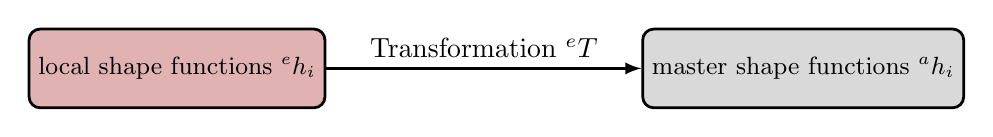
\begin{tikzpicture}
              % Draw first rectangle with PDE label
              \node[draw, rounded corners, minimum width=2cm, minimum height=1cm, fill=darkred!30,line width=1pt] (LSF) {\small local shape functions ${}^eh_i$};

              % Draw second rectangle with ODE label
              \node[draw, rounded corners, minimum width=2cm, minimum height=1cm, right=4cm of LSF, fill=gray!30,line width=1pt] (MSF) {\small  master shape functions ${}^ah_i$};

              % Draw arrow with Galerkin method label
              \draw[-latex,line width=1pt] (LSF) -- (MSF) node[midway, above] {Transformation ${}^eT$};
          \end{tikzpicture}
      \end{center}
      \begin{itemize}
          \item[\HandRight] {\color{darkred}\textbf{Clever idea:}} ${}^eT$ itself is defined in terms of archetypal shape functions and nodes coordinates:
                \[
                    {\color{darkred}{}^eT : \mathbf x(\boldxi) = {}^a\mathbf H(\boldxi) ^e{} \mathbf x=\sum_{i=1}^{{}^ep}{}^a h_i(\boldxi){}^e\mathbf x_i       }
                \]
          \item[\HandRight] Archetypal elements follows \emph{established conventions} (node numbering and nodes coordinates) that one needs to adopt.
      \end{itemize}
  \end{frame}

  \begin{frame}{The clever idea}
      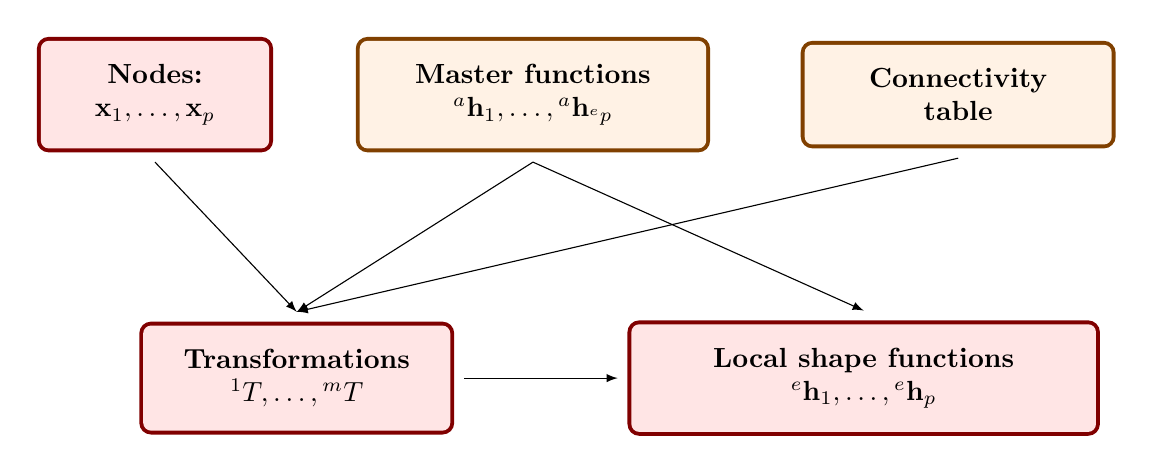
\begin{tikzpicture}[scale=0.6]
          \node (nc) at (-2,8) {
              \begin{tcolorbox}[colframe=red!50!black, colback=red!10, coltitle=black, rounded corners, width=3cm]
                  \centering \textbf{Nodes:} \\ $\mathbf x_1,\dots, \mathbf x_p$
              \end{tcolorbox}
          };
          \node (msf) at (6,8) {
              \begin{tcolorbox}[colframe=orange!50!black, colback=orange!10, coltitle=black, rounded corners,width=4.5cm]
                  \centering \textbf{Master functions} \\ ${}^a \mathbf h_1,\dots,{}^a \mathbf h_{{}^ep}$
              \end{tcolorbox}
          };
          \node (ct) at (15,8) {
              \begin{tcolorbox}[colframe=orange!50!black, colback=orange!10, coltitle=black, rounded corners,width=4cm]
                  \centering \textbf{Connectivity table}
              \end{tcolorbox}
          };
          \node (tr) at (1,2) {
              \begin{tcolorbox}[colframe=red!50!black, colback=red!10, coltitle=black, rounded corners,width=4cm]
                  \centering \textbf{Transformations} \\ ${}^1 T,\dots,{}^{m} T$
              \end{tcolorbox}
          };
          \node (sh) at (13,2) {
              \begin{tcolorbox}[colframe=red!50!black, colback=red!10, coltitle=black, rounded corners,width=6cm]
                  \centering \textbf{Local shape functions} \\ ${}^e \mathbf h_1,\dots,{}^e \mathbf h_{p}$
              \end{tcolorbox}
          };
          % Drawing arrows
          \draw[-latex, ] (nc.south) -- (tr.north);
          \draw[-latex, ] (msf.south) -- (tr.north);
          \draw[-latex, ] (ct.south) -- (tr.north);
          \draw[-latex, ] (tr.east) -- (sh.west);
          \draw[-latex, ] (msf.south) -- (sh.north);
      \end{tikzpicture}
  \end{frame}

  \begin{frame}{Concrete example: bilinear triangular element (2d)}
      \begin{columns}[T]
          \begin{column}{.45\textwidth}
              \begin{tabular}{c|c|c|c}
                  Node  id & Local                        & Node id & Global      \\
                  local    & Coord                        & global  & coord.      \\\hline
                  1        & \textcolor{darkred}{$(0,0)$} & $4$     & $(x_4,y_4)$ \\
                  2        & \textcolor{darkred}{$(1,0)$} & $8$     & $(x_8,y_8)$ \\
                  3        & \textcolor{darkred}{$(0,1)$} & $5$     & $(x_5,y_5)$ \\
              \end{tabular}
              \vspace{0.2cm}
              \newline \textbf{Base (archetypal) functions:}
              \vspace{-0.2cm}\begin{align*}
                  {}^ah_1 & = 1-\xi_1-\xi_2 \\
                  {}^ah_2 & = \xi_1         \\
                  {}^ah_3 & = \xi_2
              \end{align*}
          \end{column}
          \begin{column}{.55\textwidth}
              \vspace{0.5cm}
              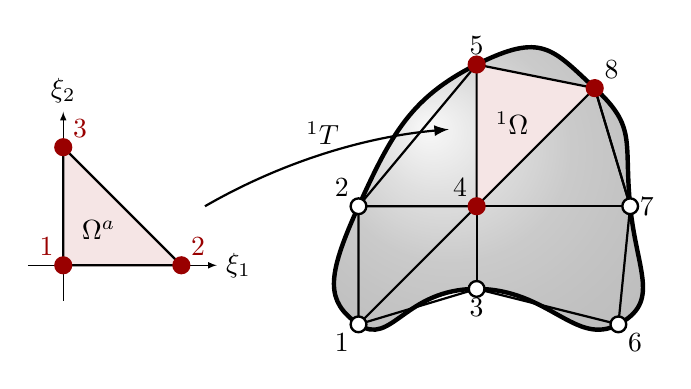
\begin{tikzpicture}[scale=1.5]
                  %\draw[step=1.0,black,thin] (-2,0) grid (4,4);
                  % Draw the potato-like shape
                  \shade [ball color= gray!90!black, opacity=.3] plot [thick,smooth cycle, tension=1] coordinates  {(1,2) (2,3.2) (3,3) (3.3,2) (3.2,1) (2,1.3) (1,1)};
                  \draw[ultra thick] plot [thick,smooth cycle, tension=1] coordinates {(1,2) (2,3.2) (3,3) (3.3,2) (3.2,1) (2,1.3) (1,1)};
                  \draw[fill=darkred!30,thick,darkred!10] (2,2) -- (3,3) -- (2,3.2) -- cycle;
                  % label the nodes
                  \node[below left] at (1,1) {$1$};
                  \node[above left] at (1,2) {$2$};
                  \node[below] at (2,1.3) {$3$};
                  \node[above left] at (2,2) {$4$};
                  \node[above] at (2,3.2) {$5$};
                  \node[below right] at (3.2,1) {$6$};
                  \node[right] at (3.3,2) {$7$};
                  \node[above right] at (3,3) {$8$};
                  % Label the region Omega
                  \node at (2.3,2.7) {${}^1\Omega$};
                  \draw[thick] (1,2) -- (2,3.2) -- (3,3) -- (3.3,2) -- (3.2,1) -- (2,1.3) -- (1,1) -- cycle;
                  \draw[thick] (1,2) -- (2,2) -- (3,3) -- (3.3,2);
                  \draw[thick] (2,1.3) -- (2,2) -- (3.3,2);
                  \draw[thick] (1,1) -- (2,2) -- (2,2.3) -- (2,3.2);
                  \node[darkred,draw,shape=circle,fill=darkred,minimum size=2mm,line width=0.3mm,inner sep=0] at (2,2) {};
                  \node[draw,shape=circle,fill=white,minimum size=2mm,line width=0.3mm,inner sep=0] at (1,1) {};
                  \node[draw,shape=circle,fill=white,minimum size=2mm,line width=0.3mm,inner sep=0] at (1,2) {};
                  \node[draw,shape=circle,fill=white,minimum size=2mm,line width=0.3mm,inner sep=0] at (2,1.3) {};
                  \node[darkred,draw,shape=circle,fill=darkred,minimum size=2mm,line width=0.3mm,inner sep=0] at (2,3.2) {};
                  \node[darkred,draw,shape=circle,fill=darkred,minimum size=2mm,line width=0.3mm,inner sep=0] at (3,3) {};
                  \node[draw,shape=circle,fill=white,minimum size=2mm,line width=0.3mm,inner sep=0] at (3.2,1) {};
                  \node[draw,shape=circle,fill=white,minimum size=2mm,line width=0.3mm,inner sep=0] at (3.3,2) {};
                  % Draw master triangle
                  \draw[fill=darkred!30,thick,darkred!10] (-1.5,1.5) -- (-0.5,1.5) -- (-1.5,2.5) -- cycle;
                  \draw[thick] (-1.5,1.5) -- (-0.5,1.5) -- (-1.5,2.5) -- cycle;
                  \draw[ultra thin,-latex] (-1.8,1.5) -- (-0.2,1.5) node[right]{$\xi_1$};
                  \draw[ultra thin,-latex] (-1.5,1.2) -- (-1.5,2.8) node[above]{$\xi_2$};
                  \node[darkred,draw,shape=circle,fill=darkred,minimum size=2mm,line width=0.3mm,inner sep=0] at (-1.5,1.5) {};
                  \node[darkred,draw,shape=circle,fill=darkred,minimum size=2mm,line width=0.3mm,inner sep=0] at (-0.5,1.5) {};
                  \node[darkred,draw,shape=circle,fill=darkred,minimum size=2mm,line width=0.3mm,inner sep=0] at (-1.5,2.5) {};
                  \node[darkred,above left] at (-1.5,1.5) {$1$};
                  \node[darkred,above right] at (-0.5,1.5) {$2$};
                  \node[darkred,above right] at (-1.5,2.5) {$3$};
                  \node at (-1.2,1.8) {$\Omega^a$};
                  \draw[thick,-latex] (-0.3,2) arc [start angle=120, end angle=95, radius=5] node[midway, above]{${}^1T$};
              \end{tikzpicture}
          \end{column}
      \end{columns}
      \vspace{0.2cm}
      \hspace{-0.3cm}\textbf{Transformation:}
      $${}^1T:\begin{cases*}
              x(\xi_1,\xi_2) =  x_4 h_1 + x_8 h_2 + x_5 h_3  = x_4+(x_8-x_4)\xi_1+(x_5-x_4)\xi_2 \\
              y(\xi_1,\xi_2)=  y_4 h_1 + y_8 h_2 + y_5 h_3 = y_4+(y_8-y_4)\xi_1+(y_5-y_4)\xi_2
          \end{cases*}$$
  \end{frame}

  \begin{frame}{\emph{Consequence 1}: explicit use of local shape functions is avoided}
      \vspace{-0.4cm}
      \begin{columns}[T,onlytextwidth]
          \begin{column}{0.56\textwidth}
              \begin{itemize}
                  \item The coordinate transformation ${}^eT^{-1}$ maps shape functions on ${}^e\Omega$ to the master element space $\Omega^a$:
                        \[
                            {}^e\mathbf H(\mathbf x)
                            =
                            {}^a\mathbf H({}^eT^{-1}(\mathbf x))
                        \]
                  \item An example of a relationship between local and archetypal shape functions:
                        \[
                            {}^1h_8(x,y)
                            =
                            {}^ah_2\big({}^1T^{-1}(x,y)\big)
                            =
                            {}^ah_2\big(\xi_1(x,y),\xi_2(x,y)\big)
                        \]
              \end{itemize}
          \end{column}

          \begin{column}{0.42\textwidth}
              \centering
              \vspace{0.4cm}
              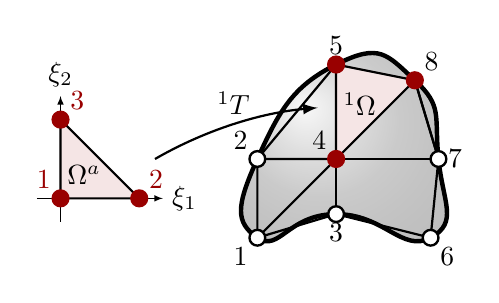
\begin{tikzpicture}[scale=1]
                  % Draw the potato-like shape
                  \shade [ball color=gray!90!black, opacity=.3]
                  plot [thick,smooth cycle, tension=1]
                  coordinates {(1,2) (2,3.2) (3,3) (3.3,2) (3.2,1) (2,1.3) (1,1)};

                  \draw[ultra thick]
                  plot [thick,smooth cycle, tension=1]
                  coordinates {(1,2) (2,3.2) (3,3) (3.3,2) (3.2,1) (2,1.3) (1,1)};

                  \draw[fill=darkred!30,thick,darkred!10] (2,2) -- (3,3) -- (2,3.2) -- cycle;

                  % Label the nodes
                  \node[below left] at (1,1) {$1$};
                  \node[above left] at (1,2) {$2$};
                  \node[below] at (2,1.3) {$3$};
                  \node[above left] at (2,2) {$4$};
                  \node[above] at (2,3.2) {$5$};
                  \node[below right] at (3.2,1) {$6$};
                  \node[right] at (3.3,2) {$7$};
                  \node[above right] at (3,3) {$8$};
                  \node at (2.3,2.7) {${}^1\Omega$};

                  \draw[thick] (1,2) -- (2,3.2) -- (3,3) -- (3.3,2)
                  -- (3.2,1) -- (2,1.3) -- (1,1) -- cycle;
                  \draw[thick] (1,2) -- (2,2) -- (3,3) -- (3.3,2);
                  \draw[thick] (2,1.3) -- (2,2) -- (3.3,2);
                  \draw[thick] (1,1) -- (2,2) -- (2,2.3) -- (2,3.2);

                  \node[darkred,draw,shape=circle,fill=darkred,minimum size=2mm,
                      line width=0.3mm,inner sep=0] at (2,2) {};
                  \node[draw,shape=circle,fill=white,minimum size=2mm,
                      line width=0.3mm,inner sep=0] at (1,1) {};
                  \node[draw,shape=circle,fill=white,minimum size=2mm,
                      line width=0.3mm,inner sep=0] at (1,2) {};
                  \node[draw,shape=circle,fill=white,minimum size=2mm,
                      line width=0.3mm,inner sep=0] at (2,1.3) {};
                  \node[darkred,draw,shape=circle,fill=darkred,minimum size=2mm,
                      line width=0.3mm,inner sep=0] at (2,3.2) {};
                  \node[darkred,draw,shape=circle,fill=darkred,minimum size=2mm,
                      line width=0.3mm,inner sep=0] at (3,3) {};
                  \node[draw,shape=circle,fill=white,minimum size=2mm,
                      line width=0.3mm,inner sep=0] at (3.2,1) {};
                  \node[draw,shape=circle,fill=white,minimum size=2mm,
                      line width=0.3mm,inner sep=0] at (3.3,2) {};

                  % Master triangle
                  \draw[fill=darkred!30,thick,darkred!10]
                  (-1.5,1.5) -- (-0.5,1.5) -- (-1.5,2.5) -- cycle;
                  \draw[thick] (-1.5,1.5) -- (-0.5,1.5) -- (-1.5,2.5) -- cycle;
                  \draw[ultra thin,-latex] (-1.8,1.5) -- (-0.2,1.5) node[right] {$\xi_1$};
                  \draw[ultra thin,-latex] (-1.5,1.2) -- (-1.5,2.8) node[above] {$\xi_2$};

                  \node[darkred,draw,shape=circle,fill=darkred,minimum size=2mm,
                      line width=0.3mm,inner sep=0] at (-1.5,1.5) {};
                  \node[darkred,draw,shape=circle,fill=darkred,minimum size=2mm,
                      line width=0.3mm,inner sep=0] at (-0.5,1.5) {};
                  \node[darkred,draw,shape=circle,fill=darkred,minimum size=2mm,
                      line width=0.3mm,inner sep=0] at (-1.5,2.5) {};
                  \node[darkred,above left] at (-1.5,1.5) {$1$};
                  \node[darkred,above right] at (-0.5,1.5) {$2$};
                  \node[darkred,above right] at (-1.5,2.5) {$3$};
                  \node at (-1.2,1.8) {$\Omega^a$};
                  \draw[thick,-latex] (-0.3,2) arc[start angle=120,end angle=95,radius=5]
                  node[midway,above] {${}^1T$};
              \end{tikzpicture}
          \end{column}
      \end{columns}

      \begin{tcolorbox}[colback=darkred!10,colframe=darkred!40!black]
          \begin{itemize}
              \item[\HandRight] In general, the inverse transformations
                    ${}^eT^{-1}:\big(\xi_1(x,y),\xi_2(x,y)\big)$ are not easy to compute
                    since the expressions in $\mathbf x(\boldsymbol{\xi})$ are nonlinear.
              \item[\HandRight] Although the local functions ${}^e h_j$ can have
                    intricate expressions, their explicit computation is not required!
          \end{itemize}
      \end{tcolorbox}

  \end{frame}

  \begin{frame}{\emph{Consequence 2}: integration over archetypal elements}
      Thanks to ${}^eT$, the integrals over ${}^e\Omega$ in the definitions of elementary stiffness and mass matrices and elementary loads vectors can be computed over the regular element $\Omega{}^a$ by performing a change of variables:
      \begin{align*}
          \int_{{\color{darkred}{}^e\Omega}}(\dots)d\Omega & \quad{\color{darkred}\xmapsto[]{\text{replaced by}}}\quad\int_{{\color{darkred}\Omega{}^a}}(\dots)\, {}^ej d\xi_1d\xi_2                                         \\[5pt]
          \frac{\partial}{\partial x_i}                    & \quad{\color{darkred}\xmapsto[]{\text{replaced by}}}\quad\frac{\partial\xi_1}{\partial x_i}\partial_{\xi_1}+ \frac{\partial\xi_2}{\partial x_i}\partial_{\xi_2}
      \end{align*}
      where ${}^ej$ is the determinant of the Jacobian matrix ${}^e\mathbf J$ of the transformation ${}^eT$.
      \vspace{0.2cm}
      \begin{tcolorbox}[colback=darkred!10,colframe=darkred!40!black,]
          \begin{itemize}
              \item[\HandRight] \small For each element, it is necessary to compute the transformation, the Jacobian matrix, its determinant, and its inverse.
          \end{itemize}
      \end{tcolorbox}
  \end{frame}

  \begin{frame}{Concrete example: bilinear triangular element (2d)}
      \begin{itemize}
          \item\textbf{Transformation:}
                $${}^1T:\begin{cases*}
                        x(\xi_1,\xi_2) =  x_4 h_1 + x_8 h_2 + x_5 h_3  = x_4+(x_8-x_4)\xi_1+(x_5-x_4)\xi_2 \\
                        y(\xi_1,\xi_2)=  y_4 h_1 + y_8 h_2 + y_5 h_3 = y_4+(y_8-y_4)\xi_1+(y_5-y_4)\xi_2
                    \end{cases*}$$
          \item \textbf{Jacobian matrix:}
                $${}^1\mathbf J=\begin{bmatrix}
                        \partial x/\partial \xi_1 & \partial x/\partial \xi_2 \\
                        \partial y/\partial \xi_1 & \partial y/\partial \xi_2
                    \end{bmatrix}=\begin{bmatrix}
                        x_8-x_4 & x_5-x_4 \\
                        y_8-y_4 & y_5-y_4
                    \end{bmatrix}$$
          \item\textbf{Jacobian determinant:} $${}^1j=\det{{}^1\mathbf J}=(x_8-x_4)( y_5-y_4)-(x_5-x_4)( y_8-y_4)$$
          \item \textbf{Jacobian inverse matrix:}
                $${}^1\mathbf J^{-1}=\frac{1}{{}^1j}\begin{bmatrix}
                        x_8-x_4  & -x_5+x_4 \\
                        -y_8+y_4 & y_5-y_4
                    \end{bmatrix}$$
      \end{itemize}
  \end{frame}

  \begin{frame}{Concrete example: bilinear triangular element (2d)}
      \begin{itemize}
          \item\textbf{Local mass matrix:}
                \begin{align*}
                    {}^1\mathbf M & =\int_{\Omega^a} \rho\, {}^a\mathbf H^T{}^a\mathbf H \, {}^1j \, d\boldxi                                 \\
                                  & = \int_{\Omega^a} \rho\begin{bmatrix}
                                                              {}^a h_1^2 \mathbf I      & {}^a h_1{}^a h_2 \mathbf I & {}^a h_1{}^a h_3 \mathbf I \\
                                                              {}^ah_2{}^a h_1 \mathbf I & {}^a h_2^2 \mathbf I       & {}^a h_2{}^a h_3 \mathbf I \\
                                                              {}^ah_3{}^a h_1 \mathbf I & {}^a h_3{}^a h_2 \mathbf I & {}^a h_3^2 \mathbf I       \\
                                                          \end{bmatrix} \, {}^1j \, d\xi_2d\xi_1
                \end{align*}

          \item \textbf{Local stiffness matrix:}
                $$
                    {}^1\mathbf K = \int_{\Omega^a} \begin{bmatrix}
                        \dots &                                                                                                                                                      & \dots \\
                              & \left({}^1\mathbf J^{-1}\boldsymbol{\nabla}_{\boldxi}{}^ah_i \right)^T\mathbf C\left( {}^1\mathbf J^{-1}\boldsymbol{\nabla}_{\boldxi}{}^ah_j \right) &       \\
                        \dots &                                                                                                                                                      & \dots \\
                    \end{bmatrix} \, {}^1j \, d\xi_2d\xi_1
                $$
      \end{itemize}
  \end{frame}

  \begin{frame}{Assembly of the mass matrix: local to global}
      \vspace{-0.7cm}
      $$
          {}^1\mathbf M
          = \int_{\Omega^a} \rho\begin{bmatrix}
              {}^a h_1^2 \mathbf I      & {}^a h_1{}^a h_2 \mathbf I & {}^a h_1{}^a h_3 \mathbf I \\
              {}^ah_2{}^a h_1 \mathbf I & {}^a h_2^2 \mathbf I       & {}^a h_2{}^a h_3 \mathbf I \\
              {}^ah_3{}^a h_1 \mathbf I & {}^a h_3{}^a h_2 \mathbf I & {}^a h_3^2 \mathbf I       \\
          \end{bmatrix} \, {}^ej \, d\xi_2d\xi_1=\begin{bmatrix}
              {}^1\mathbf M_{11} & {}^1\mathbf M_{12} & {}^1\mathbf M_{13} \\
              {}^1\mathbf M_{21} & {}^1\mathbf M_{22} & {}^1\mathbf M_{23} \\
              {}^1\mathbf M_{31} & {}^1\mathbf M_{32} & {}^1\mathbf M_{33} \\
          \end{bmatrix}$$
      We assembly local mass matrices into the global ones using the assembly operator:
      \begin{columns}
          \begin{column}{0.7\textwidth}
              \vspace{0.5cm}
              $$    \mathbf M =\A_{e=1}^m {}^e\mathbf M = \sum_{e=1}^{m} {}^e\mathbf L^T {}^e\mathbf M{}^e\mathbf L$$
              \hspace{0.7cm}where
              $${}^1\mathbf L=\begin{bmatrix}
                      \mathbf 0 & \mathbf 0 & \mathbf 0 & \mathbf I & \mathbf 0 & \mathbf 0 & \mathbf 0 & \mathbf 0 & \\
                      \mathbf 0 & \mathbf 0 & \mathbf 0 & \mathbf 0 & \mathbf 0 & \mathbf 0 & \mathbf 0 & \mathbf I & \\
                      \mathbf 0 & \mathbf 0 & \mathbf 0 & \mathbf 0 & \mathbf I & \mathbf 0 & \mathbf 0 & \mathbf 0 & \\
                  \end{bmatrix}$$
          \end{column}
          \hspace{1cm}
          \begin{column}{0.3\textwidth}
              \begin{tabular}{c|c}
                  Node  id. & Node  id. \\
                  local     & global    \\\hline
                  1         & $4$       \\
                  2         & $8$       \\
                  3         & $5$       \\
              \end{tabular}
          \end{column}
      \end{columns}
  \end{frame}

  \begin{frame}{Assembly of the mass matrix: local to global}
      $$    {}^1\mathbf L^T {}^1\mathbf M{}^1\mathbf L=\begin{bmatrix}
              \mathbf 0 & \mathbf 0 & \mathbf 0 & \mathbf 0          & \mathbf 0          & \mathbf 0 & \mathbf 0 & \mathbf 0          & \\
              \mathbf 0 & \mathbf 0 & \mathbf 0 & \mathbf 0          & \mathbf 0          & \mathbf 0 & \mathbf 0 & \mathbf 0          & \\
              \mathbf 0 & \mathbf 0 & \mathbf 0 & \mathbf 0          & \mathbf 0          & \mathbf 0 & \mathbf 0 & \mathbf 0          & \\
              \mathbf 0 & \mathbf 0 & \mathbf 0 & {}^1\mathbf M_{11} & {}^1\mathbf M_{13} & \mathbf 0 & \mathbf 0 & {}^1\mathbf M_{12} & \\
              \mathbf 0 & \mathbf 0 & \mathbf 0 & {}^1\mathbf M_{31} & {}^1\mathbf M_{33} & \mathbf 0 & \mathbf 0 & {}^1\mathbf M_{32} & \\
              \mathbf 0 & \mathbf 0 & \mathbf 0 & \mathbf 0          & \mathbf 0          & \mathbf 0 & \mathbf 0 & \mathbf 0          & \\
              \mathbf 0 & \mathbf 0 & \mathbf 0 & \mathbf 0          & \mathbf 0          & \mathbf 0 & \mathbf 0 & \mathbf 0          & \\
              \mathbf 0 & \mathbf 0 & \mathbf 0 & {}^1\mathbf M_{21} & {}^1\mathbf M_{23} & \mathbf 0 & \mathbf 0 & {}^1\mathbf M_{22} & \\
          \end{bmatrix}$$
  \end{frame}
 }


\section{3D finite elements}

\begin{frame}{Three-dimensional families of finite elements}
    \begin{center}
        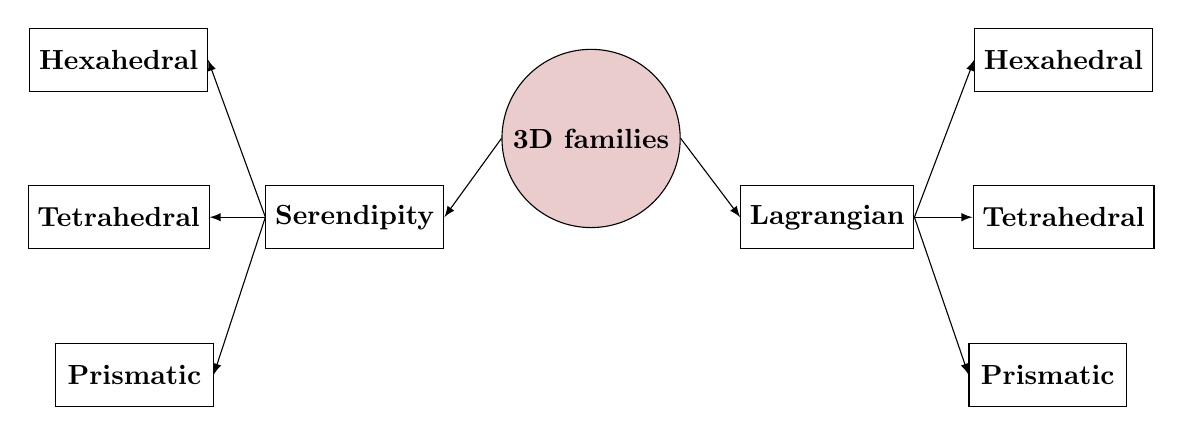
\begin{tikzpicture}
            % Draw the main circle labeled "3D"
            \node[circle, draw, minimum size=1cm, fill=darkred!20] (circle) at (0,1) {\textbf{3D families}};
            % Draw rectangles first column
            \node[draw, minimum width=2cm, minimum height=0.8cm] (hex) at (6,2) {\textbf{Hexahedral}};
            \node[draw, minimum width=2cm, minimum height=0.8cm] (tet) at (6,0) {\textbf{Tetrahedral}};
            \node[draw, minimum width=2cm, minimum height=0.8cm] (pri) at (5.8,-2) {\textbf{Prismatic}};
            \node[draw, minimum width=2cm, minimum height=0.8cm] (lag) at (3,0){\textbf{Lagrangian}};
            \node[draw, minimum width=2cm, minimum height=0.8cm] (ser) at (-3,0){\textbf{Serendipity}};
            \node[draw, minimum width=2cm, minimum height=0.8cm] (hexSer) at (-6,2) {\textbf{Hexahedral}};
            \node[draw, minimum width=2cm, minimum height=0.8cm] (tetSer) at (-6,0) {\textbf{Tetrahedral}};
            \node[draw, minimum width=2cm, minimum height=0.8cm] (priSer) at (-5.8,-2) {\textbf{Prismatic}};
            % Draw connecting arrows
            \draw[-latex] (circle.east) -- (lag.west);
            \draw[-latex] (circle.west) -- (ser.east);
            \draw[-latex] (lag.east) -- (hex.west);
            \draw[-latex] (lag.east) -- (tet.west);
            \draw[-latex] (lag.east) -- (pri.west);
            \draw[-latex] (ser.west) -- (hexSer.east);
            \draw[-latex] (ser.west) -- (tetSer.east);
            \draw[-latex] (ser.west) -- (priSer.east);
        \end{tikzpicture}
    \end{center}
\end{frame}

\begin{frame}{Serendipity vs Lagrangian elements}
    \textbf{Lagrangian finite elements}
    \begin{itemize}
        \item Defined using Lagrange polynomials.
        \item Nodes are placed at both \emph{element edges} and \emph{inside the element}.
        \item Suitable for higher-order accuracy in both structured and unstructured meshes.
    \end{itemize}

    \vspace{0.3cm}

    \textbf{Serendipity finite elements}
    \begin{itemize}
        \item Defined using a reduced number of nodes compared to Lagrangian elements.
        \item Nodes exist \emph{only on the edges} (no interior nodes for 2D elements or nodes on faces for 3D elements).
        \item More computationally efficient but less accurate for high-order approximations.
    \end{itemize}
\end{frame}

\begin{frame}{Trilinear hexahedral Lagrangian element}
    \begin{columns}
        % Left Column
        \begin{column}{0.48\textwidth}
            \vfill\centering
            \begin{tabular}{l|l}
                Node & Coordinates  \\ \hline
                1    & $(-1,-1,-1)$ \\
                2    & $(+1,-1,-1)$ \\
                3    & $(+1,+1,-1)$ \\
                4    & $(-1,+1,-1)$ \\
                5    & $(-1,-1,+1)$ \\
                6    & $(+1,-1,+1)$ \\
                7    & $(+1,+1,+1)$ \\
                8    & $(-1,+1,+1)$ \\
            \end{tabular}
            \vfill
        \end{column}
        % Right Column
        \begin{column}{0.48\textwidth}
            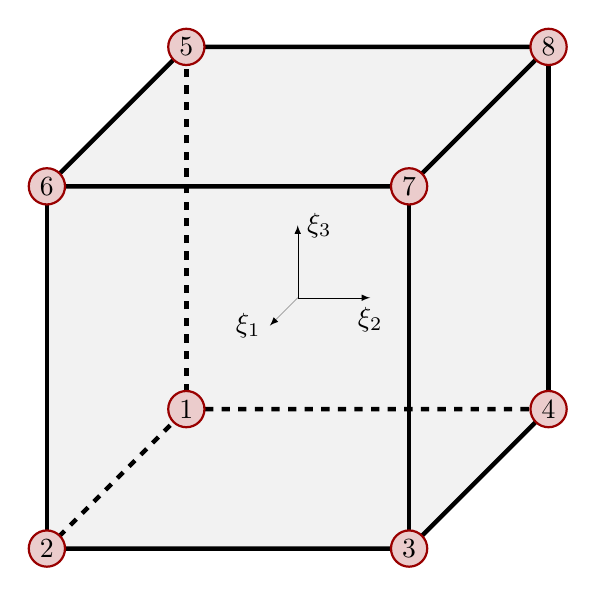
\begin{tikzpicture}[scale=2.3]
                \def\a{1}
                \coordinate (x1) at (-\a, -\a,-\a);
                \coordinate (x4) at (\a, -\a,-\a);
                \coordinate (x8) at (\a, \a,-\a);
                \coordinate (x5) at (-\a, \a,-\a);
                \coordinate (x2) at (-\a, -\a,\a);
                \coordinate (x3) at (\a, -\a,\a);
                \coordinate (x7) at (\a, \a,\a);
                \coordinate (x6) at (-\a, \a,\a);
                %Shade
                \filldraw[gray!10] (x1) -- (x2) -- (x3) -- (x4) -- cycle;
                \filldraw[gray!10] (x2) -- (x3) -- (x7) -- (x6) -- cycle;
                \filldraw[gray!10] (x3) -- (x4) -- (x8) -- (x7) -- cycle;
                \filldraw[gray!10] (x6) -- (x7) -- (x8) -- (x5) -- cycle;
                %Axis
                %Axis
                \draw[-latex,ultra thin] (0,0,0) -- (0.4,0,0) node[below]{$\xi_2$};
                \draw[-latex,ultra thin] (0,0,0) -- (0,0.4,0) node[right]{$\xi_3$};
                \draw[-latex,ultra thin] (0,0,0) -- (0,0,0.4) node[left]{$\xi_1$};
                %Draw edges
                \draw[ultra thick] (x6) -- (x7) -- (x8) -- (x5) -- cycle;
                \draw[ultra thick] (x2) -- (x3) -- (x4);
                \draw[ultra thick,dashed] (x2) -- (x1) -- (x4);
                \draw[ultra thick] (x2) -- (x6);
                \draw[ultra thick] (x3) -- (x7);
                \draw[ultra thick] (x4) -- (x8);
                \draw[ultra thick,dashed] (x1) -- (x5);
                %Draw nodes
                \draw[fill=darkred!20, thick,draw=darkred] (x1) node{1} circle(0.1cm);
                \draw[fill=darkred!20, thick,draw=darkred] (x2) node{2} circle(0.1cm);
                \draw[fill=darkred!20, thick,draw=darkred] (x3) node{3} circle(0.1cm);
                \draw[fill=darkred!20, thick,draw=darkred] (x4) node{4} circle(0.1cm);
                \draw[fill=darkred!20, thick,draw=darkred] (x5) node{5} circle(0.1cm);
                \draw[fill=darkred!20, thick,draw=darkred] (x6) node{6} circle(0.1cm);
                \draw[fill=darkred!20, thick,draw=darkred] (x7) node{7} circle(0.1cm);
                \draw[fill=darkred!20, thick,draw=darkred] (x8) node{8} circle(0.1cm);
            \end{tikzpicture}
        \end{column}
    \end{columns}
\end{frame}

\begin{frame}{Base functions for trilinear Lagrangian hexahedral elements}
    \begin{align*}
        {}^ah_1= 0.125 (1-\xi_1)(1-\xi_2)(1-\xi_3) \\
        {}^ah_2= 0.125 (1+\xi_1)(1-\xi_2)(1-\xi_3) \\
        {}^ah_3= 0.125 (1+\xi_1)(1+\xi_2)(1-\xi_3) \\
        {}^ah_4= 0.125 (1-\xi_1)(1+\xi_2)(1-\xi_3) \\
        {}^ah_5= 0.125 (1-\xi_1)(1-\xi_2)(1+\xi_3) \\
        {}^ah_6= 0.125 (1+\xi_1)(1-\xi_2)(1+\xi_3) \\
        {}^ah_7= 0.125 (1+\xi_1)(1+\xi_2)(1+\xi_3) \\
        {}^ah_8= 0.125 (1-\xi_1)(1+\xi_2)(1+\xi_3) \\
    \end{align*}
\end{frame}

\begin{frame}{Triquadratic hexahedral elements}
    \vspace{-0.5cm}
    \begin{minipage}[t]{0.48\textwidth}
        \centering
        \textbf{Lagrangian}
        \vspace{0.5cm}

        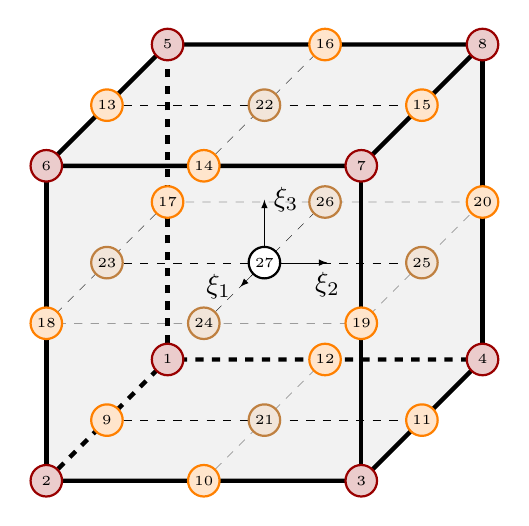
\begin{tikzpicture}[scale=2]
            \def\a{1}
            \coordinate (x1) at (-\a, -\a,-\a);
            \coordinate (x9) at (-\a, -\a,0);
            \coordinate (x2) at (-\a, -\a,\a);
            \coordinate (x10) at (0, -\a,\a);
            \coordinate (x3) at (\a, -\a,\a);
            \coordinate (x11) at (\a, -\a,0);
            \coordinate (x4) at (\a, -\a,-\a);
            \coordinate (x12) at (0, -\a,-\a);
            \coordinate (x5) at (-\a, \a,-\a);
            \coordinate (x13) at (-\a, \a,0);
            \coordinate (x6) at (-\a, \a,\a);
            \coordinate (x14) at (0, \a,\a);
            \coordinate (x7) at (\a, \a,\a);
            \coordinate (x15) at (\a, \a,0);
            \coordinate (x8) at (\a, \a,-\a);
            \coordinate (x16) at (0, \a,-\a);
            \coordinate (x17) at (-\a, 0,-\a);
            \coordinate (x18) at (-\a, 0,\a);
            \coordinate (x19) at (\a, 0,\a);
            \coordinate (x20) at (\a, 0,-\a);
            \coordinate (x21) at (0, -\a,0);
            \coordinate (x22) at (0, \a,0);
            \coordinate (x23) at (-\a, 0,0);
            \coordinate (x24) at (0, 0,\a);
            \coordinate (x25) at (\a, 0,0);
            \coordinate (x26) at (0, 0,-\a);
            \coordinate (x27) at (0,0,0);
            %Shade
            \filldraw[gray!10] (x1) -- (x2) -- (x3) -- (x4) -- cycle;
            \filldraw[gray!10] (x2) -- (x3) -- (x7) -- (x6) -- cycle;
            \filldraw[gray!10] (x3) -- (x4) -- (x8) -- (x7) -- cycle;
            \filldraw[gray!10] (x6) -- (x7) -- (x8) -- (x5) -- cycle;
            %Axis
            \draw[-latex,ultra thin] (0,0,0) -- (0.4,0,0) node[below]{$\xi_2$};
            \draw[-latex,ultra thin] (0,0,0) -- (0,0.4,0) node[right]{$\xi_3$};
            \draw[-latex,ultra thin] (0,0,0) -- (0,0,0.4) node[left]{$\xi_1$};
            %Draw edges
            \draw[ultra thick] (x6) -- (x7) -- (x8) -- (x5) -- cycle;
            \draw[ultra thick] (x2) -- (x3) -- (x4);
            \draw[ultra thick,dashed] (x2) -- (x1) -- (x4);
            \draw[ultra thick] (x2) -- (x6);
            \draw[ultra thick] (x3) -- (x7);
            \draw[ultra thick] (x4) -- (x8);
            \draw[ultra thick,dashed] (x1) -- (x5);
            \draw[ultra thin,dashed] (x17) -- (x18) -- (x19) -- (x20) -- (x17);
            \draw[ultra thin,dashed] (x23) -- (x25);
            \draw[ultra thin,dashed] (x24) -- (x26);
            \draw[ultra thin,dashed] (x9) -- (x11);
            \draw[ultra thin,dashed] (x10) -- (x12);
            \draw[ultra thin,dashed] (x13) -- (x15);
            \draw[ultra thin,dashed] (x14) -- (x16);
            %Draw nodes
            \draw[fill=darkred!20, thick,draw=darkred] (x1) node{\tiny 1} circle(0.1cm);
            \draw[fill=darkred!20, thick,draw=darkred] (x2) node{\tiny 2} circle(0.1cm);
            \draw[fill=darkred!20, thick,draw=darkred] (x3) node{\tiny 3} circle(0.1cm);
            \draw[fill=darkred!20, thick,draw=darkred] (x4) node{\tiny 4} circle(0.1cm);
            \draw[fill=darkred!20, thick,draw=darkred] (x5) node{\tiny 5} circle(0.1cm);
            \draw[fill=darkred!20, thick,draw=darkred] (x6) node{\tiny 6} circle(0.1cm);
            \draw[fill=darkred!20, thick,draw=darkred] (x7) node{\tiny 7} circle(0.1cm);
            \draw[fill=darkred!20, thick,draw=darkred] (x8) node{\tiny 8} circle(0.1cm);
            \draw[fill=orange!20, thick,draw=orange] (x9) node{\tiny 9} circle(0.1cm);
            \draw[fill=orange!20, thick,draw=orange] (x10) node{\tiny 10} circle(0.1cm);
            \draw[fill=orange!20, thick,draw=orange] (x11) node{\tiny 11} circle(0.1cm);
            \draw[fill=orange!20, thick,draw=orange] (x12) node{\tiny 12} circle(0.1cm);
            \draw[fill=orange!20, thick,draw=orange] (x13) node{\tiny 13} circle(0.1cm);
            \draw[fill=orange!20, thick,draw=orange] (x14) node{\tiny 14} circle(0.1cm);
            \draw[fill=orange!20, thick,draw=orange] (x15) node{\tiny 15} circle(0.1cm);
            \draw[fill=orange!20, thick,draw=orange] (x16) node{\tiny 16} circle(0.1cm);
            \draw[fill=orange!20, thick,draw=orange] (x17) node{\tiny 17} circle(0.1cm);
            \draw[fill=orange!20, thick,draw=orange] (x18) node{\tiny 18} circle(0.1cm);
            \draw[fill=orange!20, thick,draw=orange] (x19) node{\tiny 19} circle(0.1cm);
            \draw[fill=orange!20, thick,draw=orange] (x20) node{\tiny 20} circle(0.1cm);
            \draw[fill=brown!20, thick,draw=brown] (x21) node{\tiny 21} circle(0.1cm);
            \draw[fill=brown!20, thick,draw=brown] (x22) node{\tiny 22} circle(0.1cm);
            \draw[fill=brown!20, thick,draw=brown] (x23) node{\tiny 23} circle(0.1cm);
            \draw[fill=brown!20, thick,draw=brown] (x24) node{\tiny 24} circle(0.1cm);
            \draw[fill=brown!20, thick,draw=brown] (x25) node{\tiny 25} circle(0.1cm);
            \draw[fill=brown!20, thick,draw=brown] (x26) node{\tiny 26} circle(0.1cm);
            \draw[fill=white, thick] (x27) node{\tiny 27} circle(0.1cm);
        \end{tikzpicture}
    \end{minipage}\hfill
    \begin{minipage}[t]{0.48\textwidth}
        \centering
        \textbf{Serendipity}
        \vspace{0.5cm}

        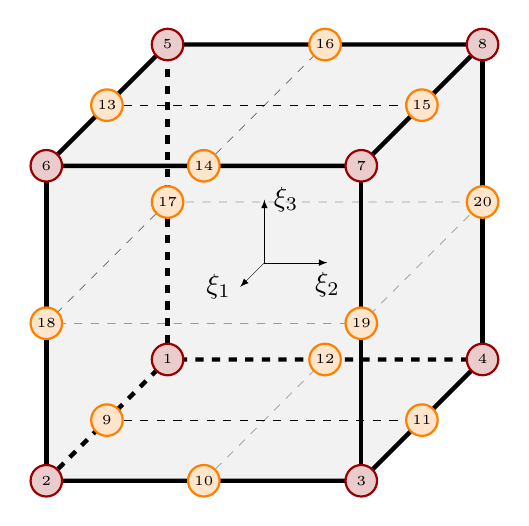
\begin{tikzpicture}[scale=2]
            \def\a{1}
            \coordinate (x1) at (-\a, -\a,-\a);
            \coordinate (x9) at (-\a, -\a,0);
            \coordinate (x2) at (-\a, -\a,\a);
            \coordinate (x10) at (0, -\a,\a);
            \coordinate (x3) at (\a, -\a,\a);
            \coordinate (x11) at (\a, -\a,0);
            \coordinate (x4) at (\a, -\a,-\a);
            \coordinate (x12) at (0, -\a,-\a);
            \coordinate (x5) at (-\a, \a,-\a);
            \coordinate (x13) at (-\a, \a,0);
            \coordinate (x6) at (-\a, \a,\a);
            \coordinate (x14) at (0, \a,\a);
            \coordinate (x7) at (\a, \a,\a);
            \coordinate (x15) at (\a, \a,0);
            \coordinate (x8) at (\a, \a,-\a);
            \coordinate (x16) at (0, \a,-\a);
            \coordinate (x17) at (-\a, 0,-\a);
            \coordinate (x18) at (-\a, 0,\a);
            \coordinate (x19) at (\a, 0,\a);
            \coordinate (x20) at (\a, 0,-\a);
            %Shade
            \filldraw[gray!10] (x1) -- (x2) -- (x3) -- (x4) -- cycle;
            \filldraw[gray!10] (x2) -- (x3) -- (x7) -- (x6) -- cycle;
            \filldraw[gray!10] (x3) -- (x4) -- (x8) -- (x7) -- cycle;
            \filldraw[gray!10] (x6) -- (x7) -- (x8) -- (x5) -- cycle;
            %Axis
            \draw[-latex,ultra thin] (0,0,0) -- (0.4,0,0) node[below]{$\xi_2$};
            \draw[-latex,ultra thin] (0,0,0) -- (0,0.4,0) node[right]{$\xi_3$};
            \draw[-latex,ultra thin] (0,0,0) -- (0,0,0.4) node[left]{$\xi_1$};
            %Draw edges
            \draw[ultra thick] (x6) -- (x7) -- (x8) -- (x5) -- cycle;
            \draw[ultra thick] (x2) -- (x3) -- (x4);
            \draw[ultra thick,dashed] (x2) -- (x1) -- (x4);
            \draw[ultra thick] (x2) -- (x6);
            \draw[ultra thick] (x3) -- (x7);
            \draw[ultra thick] (x4) -- (x8);
            \draw[ultra thick,dashed] (x1) -- (x5);
            \draw[ultra thin,dashed] (x9) -- (x11);
            \draw[ultra thin,dashed] (x10) -- (x12);
            \draw[ultra thin,dashed] (x13) -- (x15);
            \draw[ultra thin,dashed] (x14) -- (x16);
            \draw[ultra thin,dashed] (x17) -- (x18) -- (x19) -- (x20) -- cycle;
            %Draw nodes
            \draw[fill=darkred!20, thick,draw=darkred] (x1) node{\tiny 1} circle(0.1cm);
            \draw[fill=darkred!20, thick,draw=darkred] (x2) node{\tiny 2} circle(0.1cm);
            \draw[fill=darkred!20, thick,draw=darkred] (x3) node{\tiny 3} circle(0.1cm);
            \draw[fill=darkred!20, thick,draw=darkred] (x4) node{\tiny 4} circle(0.1cm);
            \draw[fill=darkred!20, thick,draw=darkred] (x5) node{\tiny 5} circle(0.1cm);
            \draw[fill=darkred!20, thick,draw=darkred] (x6) node{\tiny 6} circle(0.1cm);
            \draw[fill=darkred!20, thick,draw=darkred] (x7) node{\tiny 7} circle(0.1cm);
            \draw[fill=darkred!20, thick,draw=darkred] (x8) node{\tiny 8} circle(0.1cm);
            \draw[fill=orange!20, thick,draw=orange] (x9) node{\tiny 9} circle(0.1cm);
            \draw[fill=orange!20, thick,draw=orange] (x10) node{\tiny 10} circle(0.1cm);
            \draw[fill=orange!20, thick,draw=orange] (x11) node{\tiny 11} circle(0.1cm);
            \draw[fill=orange!20, thick,draw=orange] (x12) node{\tiny 12} circle(0.1cm);
            \draw[fill=orange!20, thick,draw=orange] (x13) node{\tiny 13} circle(0.1cm);
            \draw[fill=orange!20, thick,draw=orange] (x14) node{\tiny 14} circle(0.1cm);
            \draw[fill=orange!20, thick,draw=orange] (x15) node{\tiny 15} circle(0.1cm);
            \draw[fill=orange!20, thick,draw=orange] (x16) node{\tiny 16} circle(0.1cm);
            \draw[fill=orange!20, thick,draw=orange] (x17) node{\tiny 17} circle(0.1cm);
            \draw[fill=orange!20, thick,draw=orange] (x18) node{\tiny 18} circle(0.1cm);
            \draw[fill=orange!20, thick,draw=orange] (x19) node{\tiny 19} circle(0.1cm);
            \draw[fill=orange!20, thick,draw=orange] (x20) node{\tiny 20} circle(0.1cm);
        \end{tikzpicture}
    \end{minipage}
\end{frame}

\begin{frame}{Trilinear tetrahedral Lagrangian element}
    \begin{columns}
        % Left Column
        \begin{column}{0.48\textwidth}
            \begin{center}
                \begin{tabular}{l|l}
                    Node & Coordinates \\ \hline
                    1    & $(0,0,0)$   \\
                    2    & $(1,0,0)$   \\
                    3    & $(0,1,0)$   \\
                    4    & $(0,0,1)$   \\
                \end{tabular}
                \vspace{0.5cm}
                \newline\textbf{Base functions}
            \end{center}
            \vspace{-0.5cm}\begin{align*}
                {}^ah_1 & = 1-\xi_1-\xi_2-\xi_3 \\
                {}^ah_2 & = \xi_1               \\
                {}^ah_3 & = \xi_2               \\
                {}^ah_4 & = \xi_3               \\
            \end{align*}
        \end{column}
        % Right Column
        \begin{column}{0.48\textwidth}
            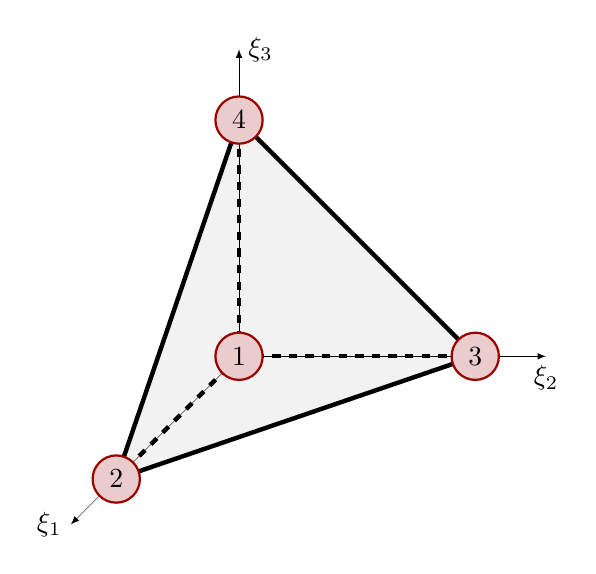
\begin{tikzpicture}[scale=3]
                \def\a{1}
                \def\b{1.35}
                \coordinate (x1) at (0,0,0);
                \coordinate (x2) at (0,0,\b);
                \coordinate (x3) at (\a,0,0);
                \coordinate (x4) at (0, \a,0);
                %Shade
                \filldraw[gray!10] (x2) -- (x3) -- (x4) -- cycle;
                %Axis
                \draw[-latex,ultra thin] (0,0,0) -- (\a+0.3,0,0) node[below]{$\xi_2$};
                \draw[-latex,ultra thin] (0,0,0) -- (0,\a+0.3,0) node[right]{$\xi_3$};
                \draw[-latex,ultra thin] (0,0,0) -- (0,0,\b+0.5) node[left]{$\xi_1$};
                %Draw edges
                \draw[ultra thick,dashed] (x1) -- (x4);
                \draw[ultra thick,dashed] (x1) -- (x2);
                \draw[ultra thick,dashed] (x1) -- (x3);
                \draw[ultra thick] (x2) -- (x3) -- (x4) -- cycle;
                %Draw nodes
                \draw[fill=darkred!20, thick,draw=darkred] (x1) node{1} circle(0.1cm);
                \draw[fill=darkred!20, thick,draw=darkred] (x2) node{2} circle(0.1cm);
                \draw[fill=darkred!20, thick,draw=darkred] (x3) node{3} circle(0.1cm);
                \draw[fill=darkred!20, thick,draw=darkred] (x4) node{4} circle(0.1cm);
            \end{tikzpicture}
        \end{column}
    \end{columns}
\end{frame}

\begin{frame}{Triquadratic tetrahedral Lagrangian element}
    \begin{columns}
        % Left Column
        \begin{column}{0.48\textwidth}
            \begin{center}
                \begin{tabular}{l|l}
                    Node & Coordinates   \\ \hline
                    1    & $(0,0,0)$     \\
                    2    & $(1,0,0)$     \\
                    3    & $(0,1,0)$     \\
                    4    & $(0,0,1)$     \\
                    5    & $(0.5,0,0)$   \\
                    6    & $(0.5,0.5,0)$ \\
                    7    & $(0,0.5,0)$   \\
                    8    & $(0,0,0.5)$   \\
                    9    & $(0.5,0,0.5)$ \\
                    10   & $(0,0.5,0.5)$ \\
                \end{tabular}
            \end{center}
        \end{column}
        % Right Column
        \begin{column}{0.48\textwidth}
            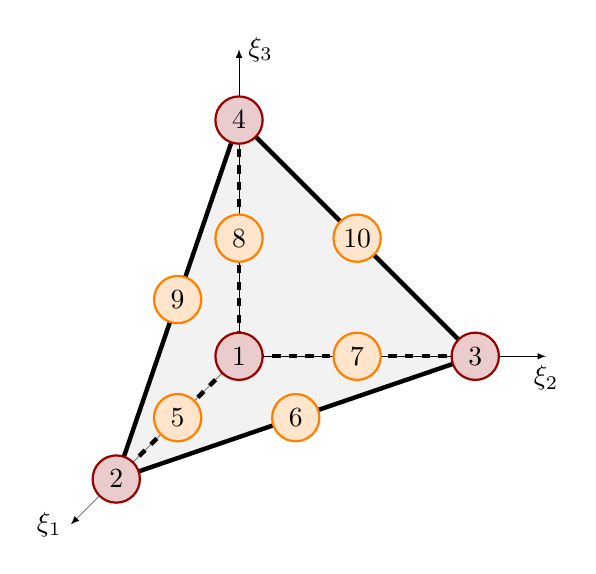
\begin{tikzpicture}[scale=3]
                \def\a{1}
                \def\b{1.35}
                \coordinate (x1) at (0,0,0);
                \coordinate (x2) at (0,0,\b);
                \coordinate (x3) at (\a,0,0);
                \coordinate (x4) at (0, \a,0);
                \coordinate (x5) at (0,0,\b/2);
                \coordinate (x6) at (\a/2,0,\b/2);
                \coordinate (x7) at (\a/2,0,0);
                \coordinate (x8) at (0,\a/2,0);
                \coordinate (x9) at (0,\a/2,\b/2);
                \coordinate (x10) at (\a/2,\a/2,0);
                %Shade
                \filldraw[gray!10] (x2) -- (x3) -- (x4) -- cycle;
                %Axis
                \draw[-latex,ultra thin] (0,0,0) -- (\a+0.3,0,0) node[below]{$\xi_2$};
                \draw[-latex,ultra thin] (0,0,0) -- (0,\a+0.3,0) node[right]{$\xi_3$};
                \draw[-latex,ultra thin] (0,0,0) -- (0,0,\b+0.5) node[left]{$\xi_1$};
                %Draw edges
                \draw[ultra thick,dashed] (x1) -- (x4);
                \draw[ultra thick,dashed] (x1) -- (x2);
                \draw[ultra thick,dashed] (x1) -- (x3);
                \draw[ultra thick] (x2) -- (x3) -- (x4) -- cycle;
                %Draw nodes
                \draw[fill=darkred!20, thick,draw=darkred] (x1) node{1} circle(0.1cm);
                \draw[fill=darkred!20, thick,draw=darkred] (x2) node{2} circle(0.1cm);
                \draw[fill=darkred!20, thick,draw=darkred] (x3) node{3} circle(0.1cm);
                \draw[fill=darkred!20, thick,draw=darkred] (x4) node{4} circle(0.1cm);
                \draw[fill=orange!20, thick,draw=orange] (x5) node{5} circle(0.1cm);
                \draw[fill=orange!20, thick,draw=orange] (x6) node{6} circle(0.1cm);
                \draw[fill=orange!20, thick,draw=orange] (x7) node{7} circle(0.1cm);
                \draw[fill=orange!20, thick,draw=orange] (x8) node{8} circle(0.1cm);
                \draw[fill=orange!20, thick,draw=orange] (x9) node{9} circle(0.1cm);
                \draw[fill=orange!20, thick,draw=orange] (x10) node{10} circle(0.1cm);
            \end{tikzpicture}
        \end{column}
    \end{columns}
\end{frame}

\begin{frame}{Triquadratic tetrahedral serendipidy element}
    \begin{columns}
        % Left Column
        \begin{column}{0.48\textwidth}
            \begin{center}
                \begin{tabular}{l|l}
                    Node & Coordinates   \\ \hline
                    1    & $(0,0,0)$     \\
                    2    & $(1,0,0)$     \\
                    3    & $(0,1,0)$     \\
                    4    & $(0,0,1)$     \\
                    5    & $(0.5,0,0)$   \\
                    6    & $(0.5,0.5,0)$ \\
                    7    & $(0,0.5,0)$   \\
                    8    & $(0.5,0,0.5)$ \\
                    9    & $(0,0.5,0.5)$ \\
                \end{tabular}
            \end{center}
        \end{column}
        % Right Column
        \begin{column}{0.48\textwidth}
            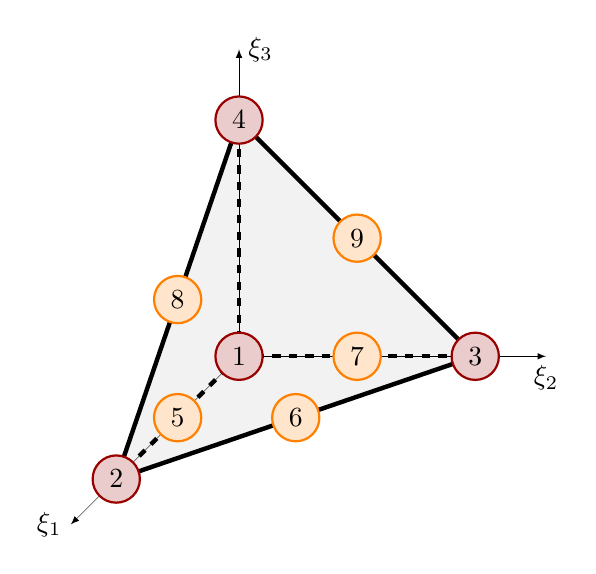
\begin{tikzpicture}[scale=3]
                \def\a{1}
                \def\b{1.35}
                \coordinate (x1) at (0,0,0);
                \coordinate (x2) at (0,0,\b);
                \coordinate (x3) at (\a,0,0);
                \coordinate (x4) at (0, \a,0);
                \coordinate (x5) at (0,0,\b/2);
                \coordinate (x6) at (\a/2,0,\b/2);
                \coordinate (x7) at (\a/2,0,0);
                \coordinate (x8) at (0,\a/2,\b/2);
                \coordinate (x9) at (\a/2,\a/2,0);
                %Shade
                \filldraw[gray!10] (x2) -- (x3) -- (x4) -- cycle;
                %Axis
                \draw[-latex,ultra thin] (0,0,0) -- (\a+0.3,0,0) node[below]{$\xi_2$};
                \draw[-latex,ultra thin] (0,0,0) -- (0,\a+0.3,0) node[right]{$\xi_3$};
                \draw[-latex,ultra thin] (0,0,0) -- (0,0,\b+0.5) node[left]{$\xi_1$};
                %Draw edges
                \draw[ultra thick,dashed] (x1) -- (x4);
                \draw[ultra thick,dashed] (x1) -- (x2);
                \draw[ultra thick,dashed] (x1) -- (x3);
                \draw[ultra thick] (x2) -- (x3) -- (x4) -- cycle;
                %Draw nodes
                \draw[fill=darkred!20, thick,draw=darkred] (x1) node{1} circle(0.1cm);
                \draw[fill=darkred!20, thick,draw=darkred] (x2) node{2} circle(0.1cm);
                \draw[fill=darkred!20, thick,draw=darkred] (x3) node{3} circle(0.1cm);
                \draw[fill=darkred!20, thick,draw=darkred] (x4) node{4} circle(0.1cm);
                \draw[fill=orange!20, thick,draw=orange] (x5) node{5} circle(0.1cm);
                \draw[fill=orange!20, thick,draw=orange] (x6) node{6} circle(0.1cm);
                \draw[fill=orange!20, thick,draw=orange] (x7) node{7} circle(0.1cm);
                \draw[fill=orange!20, thick,draw=orange] (x8) node{8} circle(0.1cm);
                \draw[fill=orange!20, thick,draw=orange] (x9) node{9} circle(0.1cm);
            \end{tikzpicture}
        \end{column}
    \end{columns}
\end{frame}

\begin{frame}{Trilinear prismatic Lagrangian element}
    \vspace{-0.2cm}
    \begin{columns}
        % Left Column
        \begin{column}{0.48\textwidth}
            \small
            \begin{center}
                \begin{tabular}{l|l}
                    Node & Coordinates \\ \hline
                    1    & $(0,0,-1)$  \\
                    2    & $(1,0,-1)$  \\
                    3    & $(0,1,-1)$  \\
                    4    & $(0,0,1)$   \\
                    5    & $(1,0,1)$   \\
                    6    & $(0,1,1)$   \\
                \end{tabular}
                \vspace{0.3cm}
                \newline\textbf{Base functions}
            \end{center}
            \vspace{-0.5cm}
            \begin{align*}
                {}^ah_1 & = (1-\xi_1-\xi_2)(1-\xi_3)/2 \\
                {}^ah_2 & = \xi_1(1-\xi_3)/2           \\
                {}^ah_3 & = \xi_2 (1-\xi_3)/2          \\
                {}^ah_4 & = (1-\xi_1-\xi_2)(1+\xi_3)/2 \\
                {}^ah_5 & = \xi_1(1+\xi_3)/2           \\
                {}^ah_6 & = \xi_2 (1+\xi_3)/2          \\
            \end{align*}
        \end{column}
        % Right Column
        \begin{column}{0.48\textwidth}
            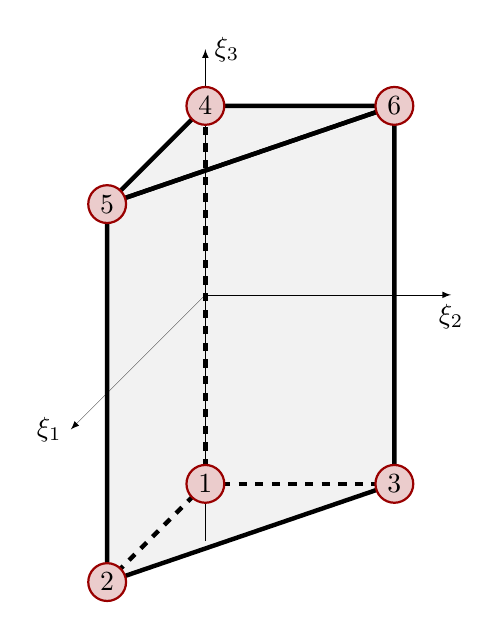
\begin{tikzpicture}[scale=2.4]
                \def\a{1}
                \def\b{1.35}
                \coordinate (x1) at (0,-\a,0);
                \coordinate (x2) at (0,-\a,\b);
                \coordinate (x3) at (\a,-\a,0);
                \coordinate (x4) at (0, \a,0);
                \coordinate (x5) at (0, \a,\b);
                \coordinate (x6) at (\a,\a,0);
                %Shade
                \filldraw[gray!10] (x2) -- (x3) -- (x6) -- (x4) -- (x5) -- (x2);
                %Axis
                \draw[-latex,ultra thin] (0,0,0) -- (\a+0.3,0,0) node[below]{$\xi_2$};
                \draw[-latex,ultra thin] (0,-\a-0.3,0) -- (0,\a+0.3,0) node[right]{$\xi_3$};
                \draw[-latex,ultra thin] (0,0,0) -- (0,0,\b+0.5) node[left]{$\xi_1$};
                %Draw edges
                \draw[ultra thick,dashed] (x1) -- (x4);
                \draw[ultra thick,dashed] (x1) -- (x2);
                \draw[ultra thick,dashed] (x1) -- (x3);
                \draw[ultra thick] (x5) -- (x4) -- (x6) -- cycle;
                \draw[ultra thick] (x6) -- (x3) -- (x2) -- (x5) -- cycle;
                %Draw nodes
                \draw[fill=darkred!20, thick,draw=darkred] (x1) node{1} circle(0.1cm);
                \draw[fill=darkred!20, thick,draw=darkred] (x2) node{2} circle(0.1cm);
                \draw[fill=darkred!20, thick,draw=darkred] (x3) node{3} circle(0.1cm);
                \draw[fill=darkred!20, thick,draw=darkred] (x4) node{4} circle(0.1cm);
                \draw[fill=darkred!20, thick,draw=darkred] (x5) node{5} circle(0.1cm);
                \draw[fill=darkred!20, thick,draw=darkred] (x6) node{6} circle(0.1cm);
            \end{tikzpicture}
        \end{column}
    \end{columns}
\end{frame}


\begin{frame}{Triquadratic prismatic elements}
    \vspace{-0.5cm}
    \begin{minipage}[t]{0.48\textwidth}
        \centering
        \textbf{Lagrangian}
        \vspace{0.5cm}


        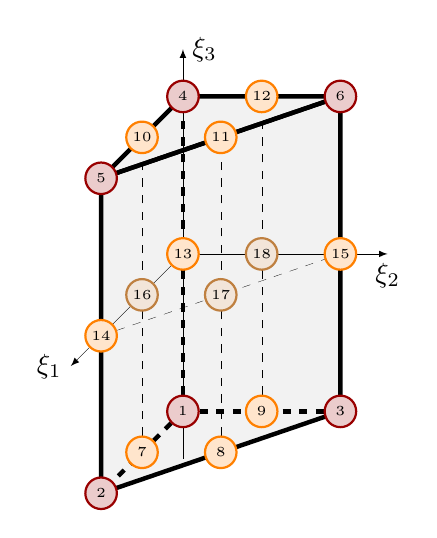
\begin{tikzpicture}[scale=2]
            \def\a{1}
            \def\b{1.35}
            \coordinate (x1) at (0,-\a,0);
            \coordinate (x2) at (0,-\a,\b);
            \coordinate (x3) at (\a,-\a,0);
            \coordinate (x4) at (0, \a,0);
            \coordinate (x5) at (0, \a,\b);
            \coordinate (x6) at (\a,\a,0);
            \coordinate (x7) at (0,-\a,\b/2);
            \coordinate (x8) at (\a/2,-\a,\b/2);
            \coordinate (x9) at (\a/2,-\a,0);
            \coordinate (x10) at (0,\a,\b/2);
            \coordinate (x11) at (\a/2,\a,\b/2);
            \coordinate (x12) at (\a/2,\a,0);
            \coordinate (x13) at (0,0,0);
            \coordinate (x14) at (0,0,\b);
            \coordinate (x15) at (\a,0,0);
            \coordinate (x16) at (0,0,\b/2);
            \coordinate (x17) at (\a/2,0,\b/2);
            \coordinate (x18) at (\a/2,0,0);
            %Shade
            \filldraw[gray!10] (x2) -- (x3) -- (x6) -- (x4) -- (x5) -- (x2);
            %Axis
            \draw[-latex,ultra thin] (0,0,0) -- (\a+0.3,0,0) node[below]{$\xi_2$};
            \draw[-latex,ultra thin] (0,-\a-0.3,0) -- (0,\a+0.3,0) node[right]{$\xi_3$};
            \draw[-latex,ultra thin] (0,0,0) -- (0,0,\b+0.5) node[left]{$\xi_1$};
            %Draw edges
            \draw[ultra thick,dashed] (x1) -- (x4);
            \draw[ultra thick,dashed] (x1) -- (x2);
            \draw[ultra thick,dashed] (x1) -- (x3);
            \draw[ultra thick] (x5) -- (x4) -- (x6) -- cycle;
            \draw[ultra thick] (x6) -- (x3) -- (x2) -- (x5) -- cycle;
            \draw[ultra thin,dashed] (x7) -- (x10);
            \draw[ultra thin,dashed] (x9) -- (x12);
            \draw[ultra thin,dashed] (x8) -- (x11);
            \draw[ultra thin,dashed] (x14) -- (x15);

            %Draw nodes
            \draw[fill=darkred!20, thick,draw=darkred] (x1) node{\tiny 1} circle(0.1cm);
            \draw[fill=darkred!20, thick,draw=darkred] (x2) node{\tiny 2} circle(0.1cm);
            \draw[fill=darkred!20, thick,draw=darkred] (x3) node{\tiny 3} circle(0.1cm);
            \draw[fill=darkred!20, thick,draw=darkred] (x4) node{\tiny 4} circle(0.1cm);
            \draw[fill=darkred!20, thick,draw=darkred] (x5) node{\tiny 5} circle(0.1cm);
            \draw[fill=darkred!20, thick,draw=darkred] (x6) node{\tiny 6} circle(0.1cm);
            \draw[fill=orange!20, thick,draw=orange] (x7) node{\tiny 7} circle(0.1cm);
            \draw[fill=orange!20, thick,draw=orange] (x8) node{\tiny 8} circle(0.1cm);
            \draw[fill=orange!20, thick,draw=orange] (x9) node{\tiny 9} circle(0.1cm);
            \draw[fill=orange!20, thick,draw=orange] (x10) node{\tiny 10} circle(0.1cm);
            \draw[fill=orange!20, thick,draw=orange] (x11) node{\tiny 11} circle(0.1cm);
            \draw[fill=orange!20, thick,draw=orange] (x12) node{\tiny 12} circle(0.1cm);
            \draw[fill=orange!20, thick,draw=orange] (x13) node{\tiny 13} circle(0.1cm);
            \draw[fill=orange!20, thick,draw=orange] (x14) node{\tiny 14} circle(0.1cm);
            \draw[fill=orange!20, thick,draw=orange] (x15) node{\tiny 15} circle(0.1cm);
            \draw[fill=brown!20, thick,draw=brown] (x16) node{\tiny 16} circle(0.1cm);
            \draw[fill=brown!20, thick,draw=brown] (x17) node{\tiny 17} circle(0.1cm);
            \draw[fill=brown!20, thick,draw=brown] (x18) node{\tiny 18} circle(0.1cm);
        \end{tikzpicture}
    \end{minipage}\hfill
    \begin{minipage}[t]{0.48\textwidth}
        \centering
        \textbf{Serendipity}
        \vspace{0.5cm}

        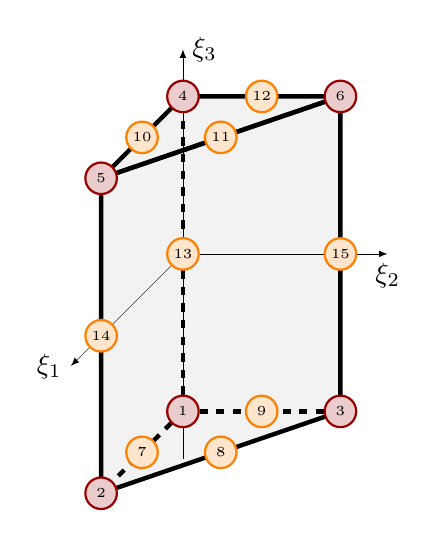
\begin{tikzpicture}[scale=2]
            \def\a{1}
            \def\b{1.35}
            \coordinate (x1) at (0,-\a,0);
            \coordinate (x2) at (0,-\a,\b);
            \coordinate (x3) at (\a,-\a,0);
            \coordinate (x4) at (0, \a,0);
            \coordinate (x5) at (0, \a,\b);
            \coordinate (x6) at (\a,\a,0);
            \coordinate (x7) at (0,-\a,\b/2);
            \coordinate (x8) at (\a/2,-\a,\b/2);
            \coordinate (x9) at (\a/2,-\a,0);
            \coordinate (x10) at (0,\a,\b/2);
            \coordinate (x11) at (\a/2,\a,\b/2);
            \coordinate (x12) at (\a/2,\a,0);
            \coordinate (x13) at (0,0,0);
            \coordinate (x14) at (0,0,\b);
            \coordinate (x15) at (\a,0,0);
            %Shade
            \filldraw[gray!10] (x2) -- (x3) -- (x6) -- (x4) -- (x5) -- (x2);
            %Axis
            \draw[-latex,ultra thin] (0,0,0) -- (\a+0.3,0,0) node[below]{$\xi_2$};
            \draw[-latex,ultra thin] (0,-\a-0.3,0) -- (0,\a+0.3,0) node[right]{$\xi_3$};
            \draw[-latex,ultra thin] (0,0,0) -- (0,0,\b+0.5) node[left]{$\xi_1$};
            %Draw edges
            \draw[ultra thick,dashed] (x1) -- (x4);
            \draw[ultra thick,dashed] (x1) -- (x2);
            \draw[ultra thick,dashed] (x1) -- (x3);
            \draw[ultra thick] (x5) -- (x4) -- (x6) -- cycle;
            \draw[ultra thick] (x6) -- (x3) -- (x2) -- (x5) -- cycle;
            %Draw nodes
            \draw[fill=darkred!20, thick,draw=darkred] (x1) node{\tiny 1} circle(0.1cm);
            \draw[fill=darkred!20, thick,draw=darkred] (x2) node{\tiny 2} circle(0.1cm);
            \draw[fill=darkred!20, thick,draw=darkred] (x3) node{\tiny 3} circle(0.1cm);
            \draw[fill=darkred!20, thick,draw=darkred] (x4) node{\tiny 4} circle(0.1cm);
            \draw[fill=darkred!20, thick,draw=darkred] (x5) node{\tiny 5} circle(0.1cm);
            \draw[fill=darkred!20, thick,draw=darkred] (x6) node{\tiny 6} circle(0.1cm);
            \draw[fill=orange!20, thick,draw=orange] (x7) node{\tiny 7} circle(0.1cm);
            \draw[fill=orange!20, thick,draw=orange] (x8) node{\tiny 8} circle(0.1cm);
            \draw[fill=orange!20, thick,draw=orange] (x9) node{\tiny 9} circle(0.1cm);
            \draw[fill=orange!20, thick,draw=orange] (x10) node{\tiny 10} circle(0.1cm);
            \draw[fill=orange!20, thick,draw=orange] (x11) node{\tiny 11} circle(0.1cm);
            \draw[fill=orange!20, thick,draw=orange] (x12) node{\tiny 12} circle(0.1cm);
            \draw[fill=orange!20, thick,draw=orange] (x13) node{\tiny 13} circle(0.1cm);
            \draw[fill=orange!20, thick,draw=orange] (x14) node{\tiny 14} circle(0.1cm);
            \draw[fill=orange!20, thick,draw=orange] (x15) node{\tiny 15} circle(0.1cm);
        \end{tikzpicture}
    \end{minipage}
\end{frame}

\section{Numerical integration}

\begin{frame}{Gauss-Legendre quadrature}
    \begin{itemize}
        \item Numerical integration helps automate the calculation of the elementary quantities ${}^e\mathbf K $, ${}^e\mathbf M$ and ${}^e\mathbf r$.
        \item Integration is approximated as:
              \begin{equation*}
                  \int_{\Omega^a}f(\boldxi) d\boldxi \approx \sum_{i=1}^{r_1} \sum_{j=1}^{r_2} \sum_{k=1}^{r_3} \omega_i^1 \omega_j^2 \omega_k^3 f(\xi_1^i, \xi_2^j, \xi_3^k)
              \end{equation*}
              where $\xi_j^i$ are known as \emph{Gauss points} and $\omega_i^j$ are their associated \emph{Gauss weights}.
    \end{itemize}
    \begin{tcolorbox}[colback=darkred!10,colframe=darkred!40!black,]
        \begin{itemize}
            \item[\HandRight]  If $f$ is a polynomial of degree $d_i=2r_i-1$ in the variable $\xi_i$, then the Gauss-Legendre approximation formula is \textbf{exact}.
        \end{itemize}
    \end{tcolorbox}
\end{frame}

\begin{frame}{Numerical integration over hexahedral solid elements}
    This allows us to compute the stiffness matrix, the mass matrix and the load vector numerically as:
    \begin{align*}
        {}^e\mathbf K & \approx\sum_{i=1}^{r_1} \sum_{j=1}^{r_2} \sum_{k=1}^{r_3} \omega_i^1 \omega_j^2 \omega_k^3 \left[ ( {}^e\mathbf J^{-1}\boldsymbol{\nabla}_{\boldxi}{}^a\mathbf H)^T \mathbf C ({}^e\mathbf J^{-1}\boldsymbol{\nabla}_{\boldxi} {}^a\mathbf H ) {}^e j \right]_{\xi_1=\xi_1^i, \xi_2=\xi_2^j, \xi_3=\xi_3^k}                                     \\[10pt]
        {}^e\mathbf M & \approx\sum_{i=1}^{r_1} \sum_{j=1}^{r_2} \sum_{k=1}^{r_3}  \omega_i^1 \omega_j^2 \omega_k^3 \left[  \rho\, {}^a\mathbf H^T{}^a\mathbf H \right]_{\xi_1=\xi_1^i, \xi_2=\xi_2^j, \xi_3=\xi_3^k}                                                                                                                                                   \\[10pt]
        {}^e\mathbf r & \approx\sum_{i=1}^{r_1} \sum_{j=1}^{r_2} \tilde\omega_i^1 \tilde\omega_j^2 \left[ {}^a\mathbf H^T\mathbf{\hat f} \right]_{\xi_1= \tilde\xi_1^i, \xi_2= \tilde\xi_2^j}+\sum_{i=1}^{r_1} \sum_{j=1}^{r_2} \sum_{k=1}^{r_3} \omega_i^1 \omega_j^2 \omega_k^3 \left[ {}^a\mathbf H^T\mathbf f \right]_{\xi_1=\xi_1^i, \xi_2=\xi_2^j, \xi_3=\xi_3^k}
    \end{align*}
\end{frame}

\begin{frame}{An illustration of Gauss points - 2d elements}
    \centering
    \begin{figure}
        \centering
        \begin{subfigure}{0.45\textwidth}
            \centering
            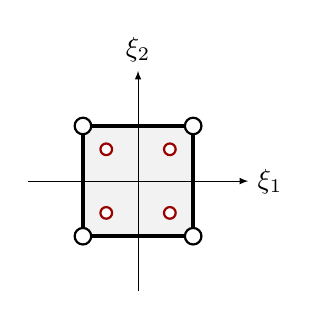
\begin{tikzpicture}[scale=0.7]
                \def\a{2}
                \def\b{2}
                \coordinate (x1) at (0, 0);
                \coordinate (x2) at (\a, 0);
                \coordinate (x3) at (0, \b);
                \coordinate (x4) at (\a, \b);
                \filldraw[gray!10] (x1) -- (x2) -- (x4) -- (x3) -- cycle;
                \draw[ultra thick] (x1) -- (x2) -- (x4) -- (x3) -- cycle;
                \draw[fill=white, thick] (x1) circle(0.15cm);
                \draw[fill=white, thick] (x2) circle(0.15cm);
                \draw[fill=white, thick] (x3) circle(0.15cm);
                \draw[fill=white, thick] (x4) circle(0.15cm);
                \draw[-latex,ultra thin] (-1,\b/2) -- (\a+1,\b/2) node[right]{$\xi_1$};
                \draw[-latex,ultra thin] (\a/2,-1) -- (\a/2,\b+1) node[above]{$\xi_2$};
                \draw[fill=white, thick, draw=darkred]  (\a/2+0.577,\b/2+0.577) circle (3pt);
                \draw[fill=white, thick, draw=darkred]  (\a/2-0.577,\b/2+0.577) circle (3pt);
                \draw[fill=white, thick, draw=darkred]  (\a/2-0.577,\b/2-0.577) circle (3pt);
                \draw[fill=white, thick, draw=darkred]  (\a/2+0.577,\b/2-0.577) circle (3pt);
            \end{tikzpicture}
        \end{subfigure}
        \hfill
        \begin{subfigure}{0.45\textwidth}
            \centering
            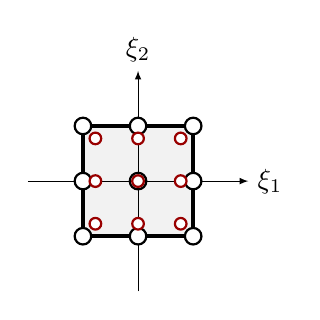
\begin{tikzpicture}[scale=0.7]
                \def\a{2}
                \def\b{2}
                \coordinate (x1) at (0, 0);
                \coordinate (x2) at (\a, 0);
                \coordinate (x3) at (0, \b);
                \coordinate (x4) at (\a, \b);
                \coordinate (x5) at (\a/2, 0);
                \coordinate (x6) at (\a, \b/2);
                \coordinate (x7) at (\a/2, \b);
                \coordinate (x8) at (0, \b/2);
                \coordinate (x9) at (\a/2, \b/2);
                \filldraw[gray!10] (x1) -- (x2) -- (x4) -- (x3) -- cycle;
                \draw[ultra thick] (x1) -- (x2) -- (x4) -- (x3) -- cycle;
                \draw[-latex,ultra thin] (-1,\b/2) -- (\a+1,\b/2) node[right]{$\xi_1$};
                \draw[-latex,ultra thin] (\a/2,-1) -- (\a/2,\b+1) node[above]{$\xi_2$};
                \draw[fill=white, thick] (x1) circle(0.15cm);
                \draw[fill=white, thick] (x2) circle(0.15cm);
                \draw[fill=white, thick] (x3) circle(0.15cm);
                \draw[fill=white, thick] (x4) circle(0.15cm);
                \draw[fill=white, thick] (x5) circle(0.15cm);
                \draw[fill=white, thick] (x6) circle(0.15cm);
                \draw[fill=white, thick] (x7) circle(0.15cm);
                \draw[fill=white, thick] (x8) circle(0.15cm);
                \draw[fill=white, thick] (x9) circle(0.15cm);
                \draw[fill=white, thick, draw=darkred]  (\a/2+0.774,\b/2+0.774) circle (3pt);
                \draw[fill=white, thick, draw=darkred]  (\a/2-0.774,\b/2-0.774) circle (3pt);
                \draw[fill=white, thick, draw=darkred]  (\a/2+0.774,\b/2-0.774) circle (3pt);
                \draw[fill=white, thick, draw=darkred]  (\a/2-0.774,\b/2+0.774) circle (3pt);
                \draw[fill=white, thick, draw=darkred]  (\a/2,\b/2+0.774) circle (3pt);
                \draw[fill=white, thick, draw=darkred]  (\a/2,\b/2-0.774) circle (3pt);
                \draw[fill=white, thick, draw=darkred]  (\a/2-0.774,\b/2) circle (3pt);
                \draw[fill=white, thick, draw=darkred]  (\a/2+0.774,\b/2) circle (3pt);
                \draw[fill=white, thick, draw=darkred]  (\a/2,\b/2) circle (3pt);
            \end{tikzpicture}
        \end{subfigure}

        \vfill

        \begin{subfigure}{0.45\textwidth}
            \centering
            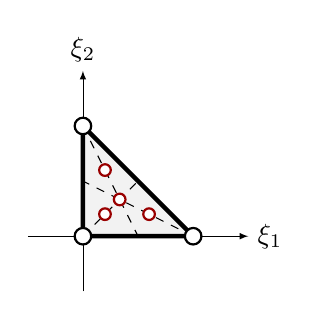
\begin{tikzpicture}[scale=0.7]
                \def\a{2}
                \def\b{2}
                \coordinate (x1) at (0, 0);
                \coordinate (x2) at (\a, 0);
                \coordinate (x3) at (0, \b);
                \filldraw[gray!10] (x1) -- (x2) -- (x3) -- cycle;
                \draw[ultra thick] (x1) -- (x2)-- (x3) -- cycle;
                \draw[-latex,ultra thin] (-1,0) -- (\a+1,0) node[right]{$\xi_1$};
                \draw[-latex,ultra thin] (0,-1) -- (0,\b+1) node[above]{$\xi_2$};
                \draw[thin, dashed] (x1) -- (\a/2,\b/2);
                \draw[thin, dashed] (x2) -- (0,\b/2);
                \draw[thin, dashed] (x3) -- (\a/2,0);
                \draw[fill=white, thick] (x1)  circle(0.15cm);
                \draw[fill=white, thick] (x2)  circle(0.15cm);
                \draw[fill=white, thick] (x3)  circle(0.15cm);
                \draw[fill=white, thick, draw=darkred]  (2*1/5,2*1/5) circle (3pt);
                \draw[fill=white, thick, draw=darkred]  (2*3/5,2*1/5) circle (3pt);
                \draw[fill=white, thick, draw=darkred]  (2*1/5,2*3/5) circle (3pt);
                \draw[fill=white, thick, draw=darkred]  (2*1/3,2*1/3) circle (3pt);
            \end{tikzpicture}
        \end{subfigure}
        \hfill
        \begin{subfigure}{0.45\textwidth}
            \centering
            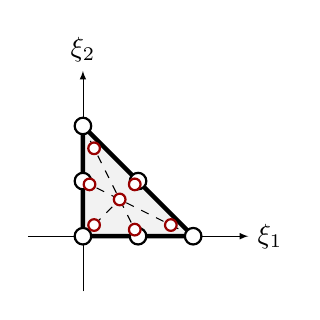
\begin{tikzpicture}[scale=0.7]
                \def\a{2}
                \def\b{2}
                \coordinate (x1) at (0, 0);
                \coordinate (x2) at (\a, 0);
                \coordinate (x3) at (0, \b);
                \coordinate (x4) at (\a/2,0);
                \coordinate (x5) at (\a/2, \b/2);
                \coordinate (x6) at (0, \b/2);
                \filldraw[gray!10] (x1) -- (x2) -- (x3) -- cycle;
                \draw[ultra thick] (x1) -- (x2)-- (x3) -- cycle;
                \draw[-latex,ultra thin] (-1,0) -- (\a+1,0) node[right]{$\xi_1$};
                \draw[-latex,ultra thin] (0,-1) -- (0,\b+1) node[above]{$\xi_2$};
                \draw[thin, dashed] (x1) -- (\a/2,\b/2);
                \draw[thin, dashed] (x2) -- (0,\b/2);
                \draw[thin, dashed] (x3) -- (\a/2,0);
                \draw[fill=white, thick] (x1)  circle(0.15cm);
                \draw[fill=white, thick] (x2)  circle(0.15cm);
                \draw[fill=white, thick] (x3)  circle(0.15cm);
                \draw[fill=white, thick] (x4)  circle(0.15cm);
                \draw[fill=white, thick] (x5)  circle(0.15cm);
                \draw[fill=white, thick] (x6)  circle(0.15cm);
                \draw[fill=white, thick, draw=darkred]  (2*0.10128,2*0.10128) circle (3pt);
                \draw[fill=white, thick, draw=darkred]  (2*0.7974,2*0.10128) circle (3pt);
                \draw[fill=white, thick, draw=darkred]  (2*0.10128,2*0.7974) circle (3pt);
                \draw[fill=white, thick, draw=darkred]  (2*0.47014,2*0.47014) circle (3pt);
                \draw[fill=white, thick, draw=darkred]  (2*0.47014,2*0.05971) circle (3pt);
                \draw[fill=white, thick, draw=darkred]  (2*0.05971,2*0.47014) circle (3pt);
                \draw[fill=white, thick, draw=darkred]  (2*0.3333,2*0.3333) circle (3pt);
            \end{tikzpicture}
        \end{subfigure}
    \end{figure}
\end{frame}

\begin{frame}{An illustration of Gauss points - 3d elements}
    \centering
    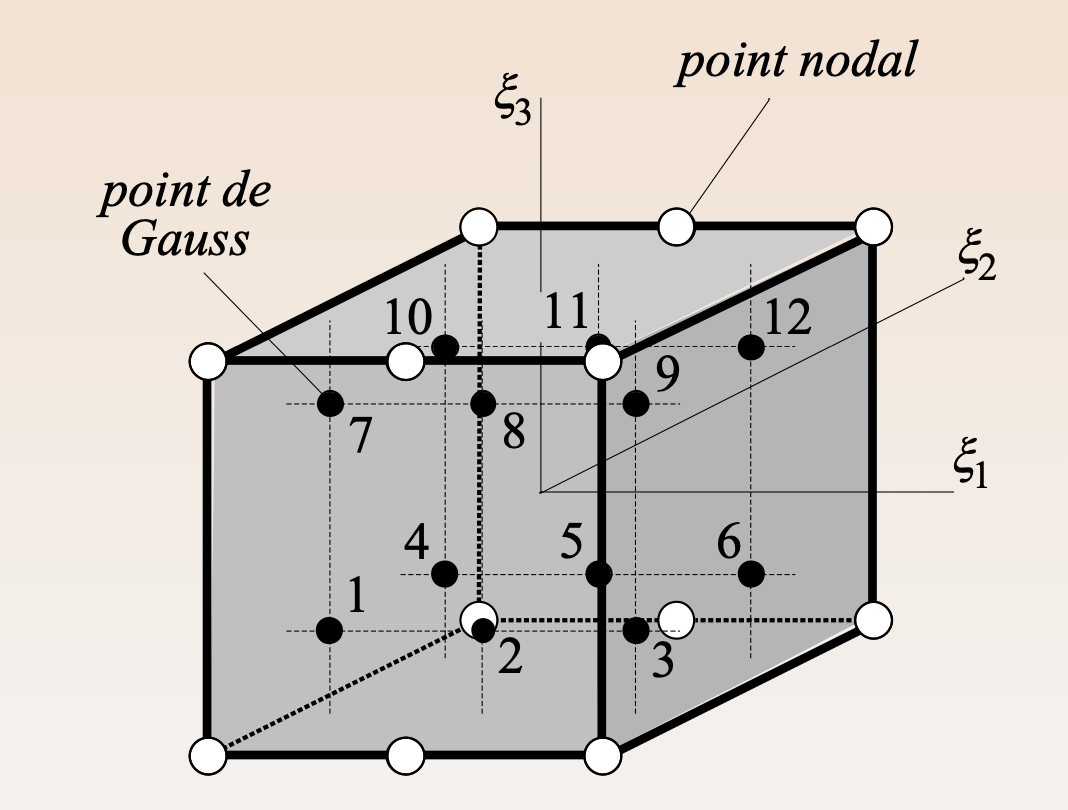
\includegraphics[height=5cm]{../images/gaussPoint1.png}\hspace{1cm}
    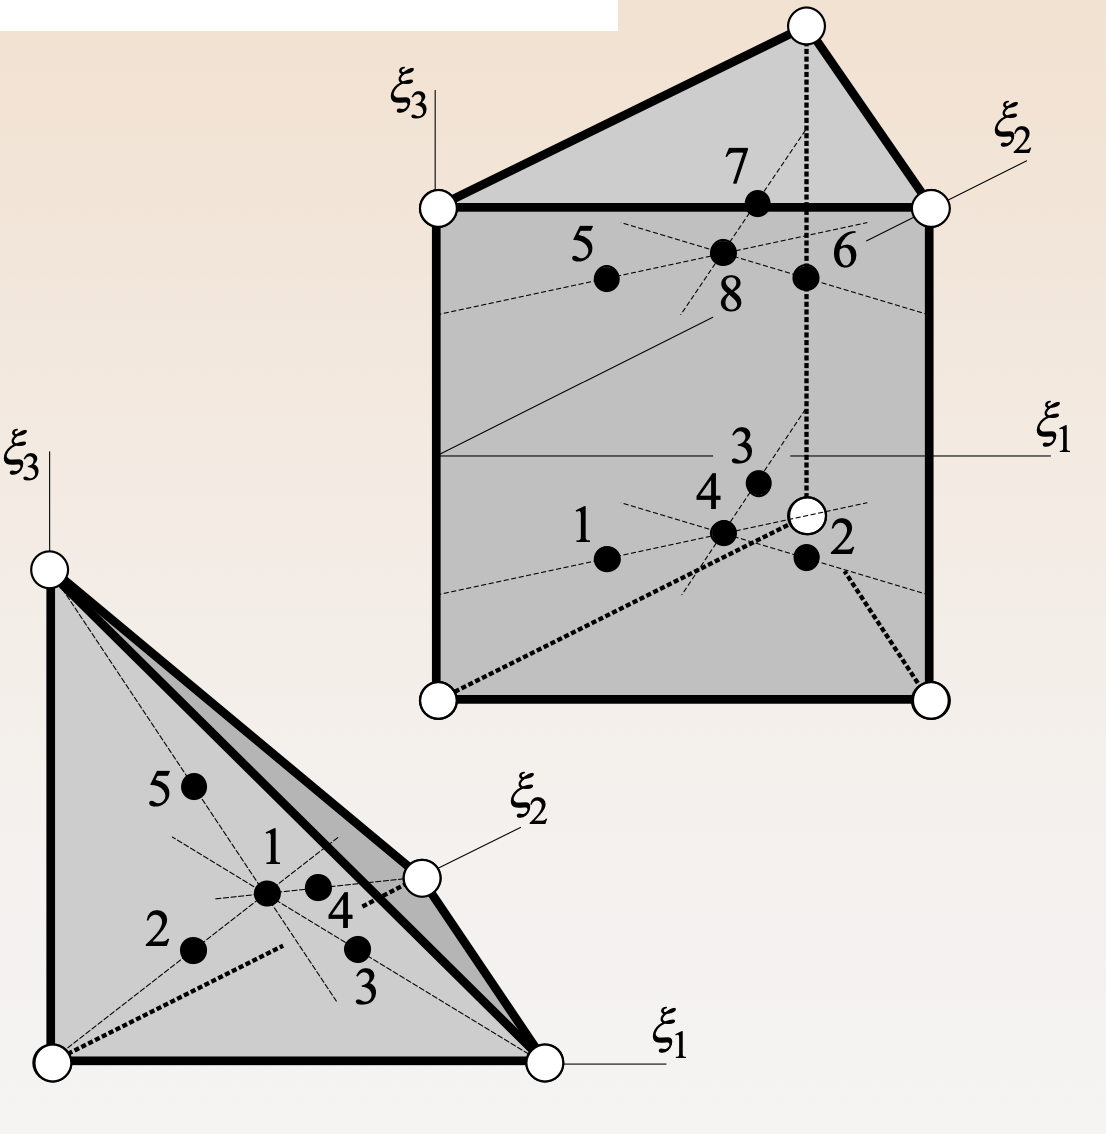
\includegraphics[height=5cm]{../images/gaussPoint2.png}
    \newline
    {\footnotesize (Credit: Thomas Gmür - Dynamique numérique des solides et des structures)}
\end{frame}

\begin{frame}{Numerical integration in 3d}
    \vspace{-0.1cm}
    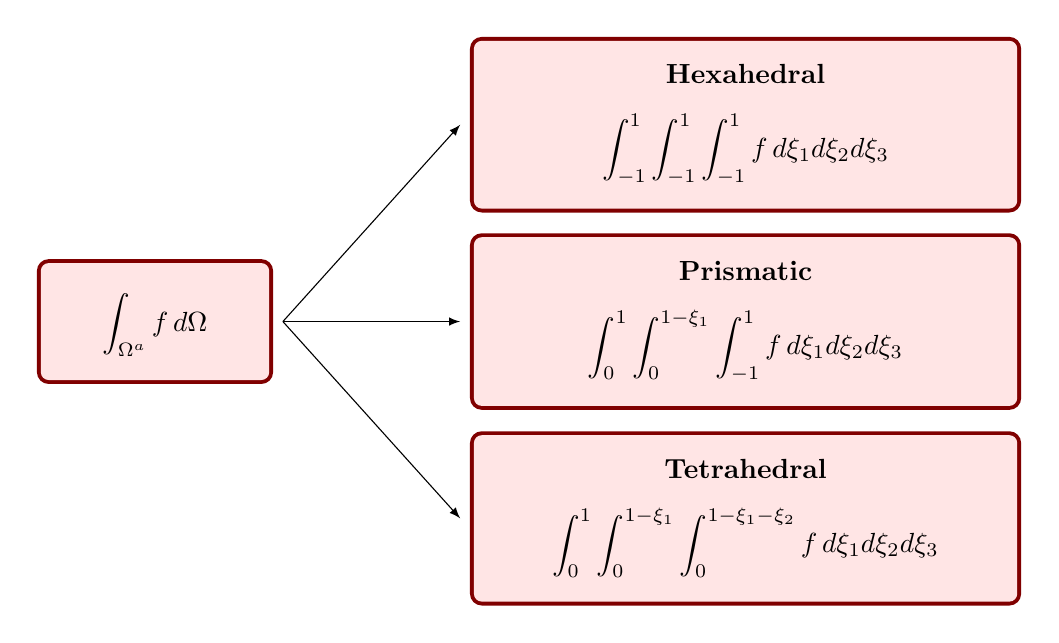
\begin{tikzpicture}[scale=0.5]
        \node (arch) at (-2,0) {
            \begin{tcolorbox}[colframe=red!50!black, colback=red!10, coltitle=black, rounded corners, width=3cm]\vspace{-0.3cm}
                $$\int_{\Omega^a} f\, d\Omega$$
            \end{tcolorbox}
        };
        \node (hex) at (13,5) {
            \begin{tcolorbox}[colframe=red!50!black, colback=red!10, coltitle=black, rounded corners,width=7cm]
                \centering \textbf{Hexahedral} $$\int_{-1}^1\int_{-1}^1\int_{-1}^1 f\, d\xi_1d\xi_2d\xi_3$$
            \end{tcolorbox}
        };
        \node (pri) at (13,0) {
            \begin{tcolorbox}[colframe=red!50!black, colback=red!10, coltitle=black, rounded corners,width=7cm]
                \centering \textbf{Prismatic} $$\int_{0}^1\int_{0}^{1-\xi_1}\int_{-1}^1 f\, d\xi_1d\xi_2d\xi_3$$
            \end{tcolorbox}
        };
        \node (tri) at (13,-5) {
            \begin{tcolorbox}[colframe=red!50!black, colback=red!10, coltitle=black, rounded corners,width=7cm]
                \centering \textbf{Tetrahedral} $$\int_{0}^1\int_{0}^{1-\xi_1}\int_{0}^{1-\xi_1-\xi_2}f\, d\xi_1d\xi_2d\xi_3$$
            \end{tcolorbox}
        };
        % Drawing arrows
        \draw[-latex, ] (arch.east) -- (hex.west);
        \draw[-latex, ] (arch.east) -- (pri.west);
        \draw[-latex, ] (arch.east) -- (tri.west);
    \end{tikzpicture}
\end{frame}

\begin{frame}{Gauss-Legendre numerical integration}
    \vspace{-0.1cm}
    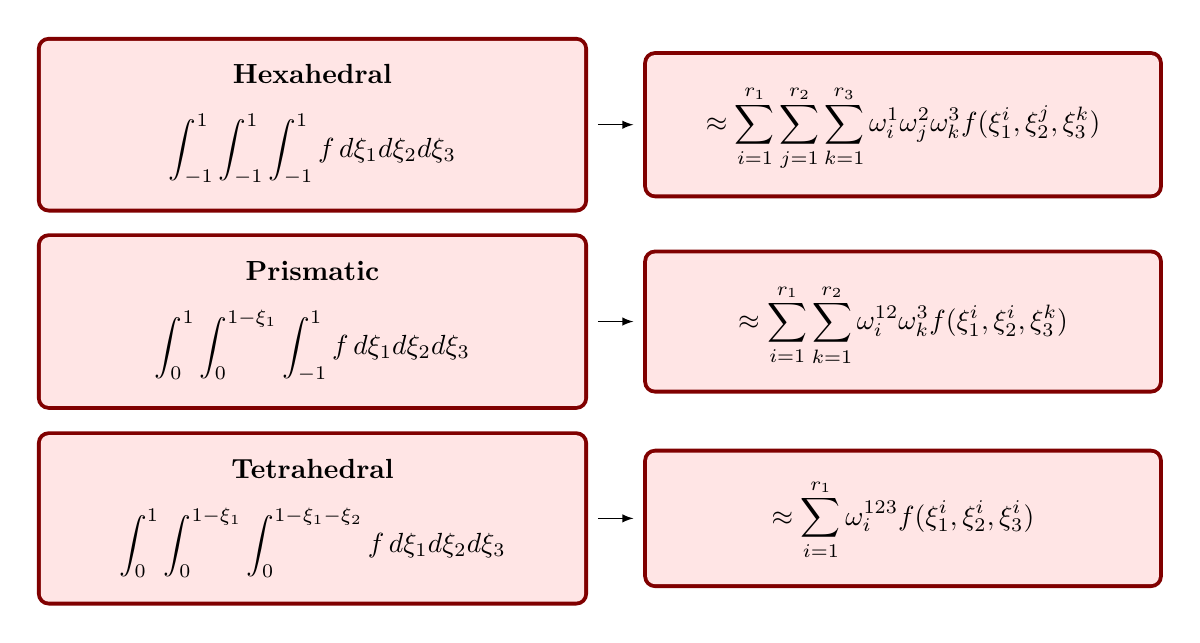
\begin{tikzpicture}[scale=0.5]
        \node (hex) at (0,5) {
            \begin{tcolorbox}[colframe=red!50!black, colback=red!10, coltitle=black, rounded corners,width=7cm]
                \centering \textbf{Hexahedral} $$\int_{-1}^1\int_{-1}^1\int_{-1}^1 f\, d\xi_1d\xi_2d\xi_3$$
            \end{tcolorbox}
        };
        \node (hexGauss) at (15,5) {
            \begin{tcolorbox}[colframe=red!50!black, colback=red!10, coltitle=black, rounded corners,width=6.6cm]
                \vspace{-0.3cm}$$\approx\sum_{i=1}^{r_1} \sum_{j=1}^{r_2} \sum_{k=1}^{r_3} \omega_i^1 \omega_j^2 \omega_k^3 f(\xi_1^i, \xi_2^j, \xi_3^k)$$
            \end{tcolorbox}
        };
        \node (pri) at (0,0) {
            \begin{tcolorbox}[colframe=red!50!black, colback=red!10, coltitle=black, rounded corners,width=7cm]
                \centering \textbf{Prismatic} $$\int_{0}^1\int_{0}^{1-\xi_1}\int_{-1}^1 f\, d\xi_1d\xi_2d\xi_3$$
            \end{tcolorbox}
        };
        \node (priGauss) at (15,0) {
            \begin{tcolorbox}[colframe=red!50!black, colback=red!10, coltitle=black, rounded corners,width=6.6cm]
                \vspace{-0.3cm}$$\approx\sum_{i=1}^{r_1} \sum_{k=1}^{r_2} \omega_i^{12}\omega_k^3 f(\xi_1^i, \xi_2^i, \xi_3^k)$$
            \end{tcolorbox}
        };
        \node (tri) at (0,-5) {
            \begin{tcolorbox}[colframe=red!50!black, colback=red!10, coltitle=black, rounded corners,width=7cm]
                \centering \textbf{Tetrahedral} $$\int_{0}^1\int_{0}^{1-\xi_1}\int_{0}^{1-\xi_1-\xi_2}f\, d\xi_1d\xi_2d\xi_3$$
            \end{tcolorbox}
        };
        \node (triGauss) at (15,-5) {
            \begin{tcolorbox}[colframe=red!50!black, colback=red!10, coltitle=black, rounded corners,width=6.6cm]
                $$\approx\sum_{i=1}^{r_1} \omega_i^{123} f(\xi_1^i, \xi_2^i, \xi_3^i)$$
            \end{tcolorbox}
        };
        % Drawing arrows
        \draw[-latex, ] (hex.east) -- (hexGauss.west);
        \draw[-latex, ] (pri.east) -- (priGauss.west);
        \draw[-latex, ] (tri.east) -- (triGauss.west);
    \end{tikzpicture}
\end{frame}


\begin{frame}{Example of numerical integration using Gauss-Legendre quadrature in 2d}
    \vspace{-0.5cm}
    \begin{equation*}
        \int_{\Omega^a}f(\xi_1,\xi_2) d\xi_1d\xi_2 \approx \sum_{i=1}^{4}  \omega_i f(\xi_1^i, \xi_2^i)
    \end{equation*}
    \vspace{-0.3cm}
    \begin{columns}[T]
        \begin{column}{.45\textwidth}
            \centering
            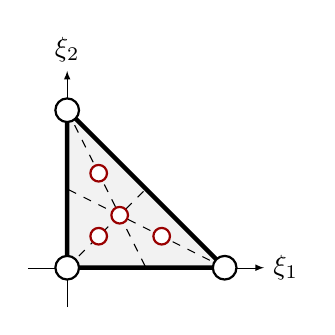
\begin{tikzpicture}[scale=1]
                \def\a{2}
                \def\b{2}
                \coordinate (x1) at (0, 0);
                \coordinate (x2) at (\a, 0);
                \coordinate (x3) at (0, \b);
                \filldraw[gray!10] (x1) -- (x2) -- (x3) -- cycle;
                \draw[ultra thick] (x1) -- (x2)-- (x3) -- cycle;
                \draw[-latex,ultra thin] (-0.5,0) -- (\a+0.5,0) node[right]{$\xi_1$};
                \draw[-latex,ultra thin] (0,-0.5) -- (0,\b+0.5) node[above]{$\xi_2$};
                \draw[thin, dashed] (x1) -- (\a/2,\b/2);
                \draw[thin, dashed] (x2) -- (0,\b/2);
                \draw[thin, dashed] (x3) -- (\a/2,0);
                \draw[fill=white, thick] (x1)  circle(0.15cm);
                \draw[fill=white, thick] (x2)  circle(0.15cm);
                \draw[fill=white, thick] (x3)  circle(0.15cm);
                \draw[fill=white, thick, draw=darkred]  (2*1/5,2*1/5) circle (3pt);
                \draw[fill=white, thick, draw=darkred]  (2*3/5,2*1/5) circle (3pt);
                \draw[fill=white, thick, draw=darkred]  (2*1/5,2*3/5) circle (3pt);
                \draw[fill=white, thick, draw=darkred]  (2*1/3,2*1/3) circle (3pt);
            \end{tikzpicture}
        \end{column}
        \begin{column}{.55\textwidth}
            \begin{tabular}{c|c}
                Gauss points ($\xi_1^i, \xi_2^i$) & Weights ($\omega_i$) \\[5pt]
                $(1/5,1/5)$                       & $25/96$              \\[5pt]
                $(3/5,1/5)$                       & $25/96$              \\[5pt]
                $(1/5,3/5)$                       & $25/96$              \\[5pt]
                $(1/3,1/3)$                       & $9/32$               \\[5pt]
            \end{tabular}
        \end{column}
    \end{columns}
    \vspace{0.5cm}
    \begin{tcolorbox}[colback=darkred!10,colframe=darkred!40!black,]
        Since we are using 2 Gauss points in each \emph{direction}, the approximation is exact for polynomials of degree up to $3$ in each variable.
    \end{tcolorbox}
\end{frame}

\begin{frame}{Number of Gauss points for exact integration}
    \begin{columns}
        \begin{column}{0.7\textwidth}
            \textbf{Trilinear hexahedral element}
            \begin{itemize}
                \item Basis functions are linear in each variable.
                \item Exact integration with:
                      \begin{itemize}
                          \item $2\times2\times2$ Gauss points for ${}^e\mathbf M$
                          \item $1\times1\times1$ Gauss points for ${}^e\mathbf K$
                      \end{itemize}
                      if the element is not distorted.
                \item Note that in case of distortion:
                      \begin{itemize}
                          \item Jacobian is a function of $\boldxi$ : ${}^ej={}^ej(\boldxi)$\vspace{0.2cm}
                          \item ${}^e\mathbf J^{-1}={}^e\mathbf J^{-1}(\boldxi)$ function of $\boldxi$ at the denominator.\vspace{0.2cm}
                          \item $\frac{\partial {}^e\mathbf H}{\partial \bold x}={}^e\mathbf J^{-1}\frac{\partial {}^a\mathbf H}{\partial \boldxi} $ is not a polynomial function of $\boldxi$ anymore.
                      \end{itemize}
            \end{itemize}
        \end{column}
        % Right Column
        \begin{column}{0.3\textwidth}
            \centering
            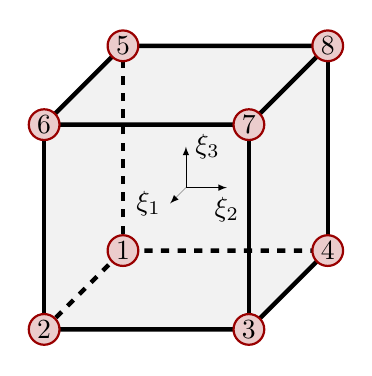
\begin{tikzpicture}[scale=1.3]
                \def\a{1}
                \coordinate (x1) at (-\a, -\a,-\a);
                \coordinate (x4) at (\a, -\a,-\a);
                \coordinate (x8) at (\a, \a,-\a);
                \coordinate (x5) at (-\a, \a,-\a);
                \coordinate (x2) at (-\a, -\a,\a);
                \coordinate (x3) at (\a, -\a,\a);
                \coordinate (x7) at (\a, \a,\a);
                \coordinate (x6) at (-\a, \a,\a);
                %Shade
                \filldraw[gray!10] (x1) -- (x2) -- (x3) -- (x4) -- cycle;
                \filldraw[gray!10] (x2) -- (x3) -- (x7) -- (x6) -- cycle;
                \filldraw[gray!10] (x3) -- (x4) -- (x8) -- (x7) -- cycle;
                \filldraw[gray!10] (x6) -- (x7) -- (x8) -- (x5) -- cycle;
                %Axis
                %Axis
                \draw[-latex,ultra thin] (0,0,0) -- (0.4,0,0) node[below]{$\xi_2$};
                \draw[-latex,ultra thin] (0,0,0) -- (0,0.4,0) node[right]{$\xi_3$};
                \draw[-latex,ultra thin] (0,0,0) -- (0,0,0.4) node[left]{$\xi_1$};
                %Draw edges
                \draw[ultra thick] (x6) -- (x7) -- (x8) -- (x5) -- cycle;
                \draw[ultra thick] (x2) -- (x3) -- (x4);
                \draw[ultra thick,dashed] (x2) -- (x1) -- (x4);
                \draw[ultra thick] (x2) -- (x6);
                \draw[ultra thick] (x3) -- (x7);
                \draw[ultra thick] (x4) -- (x8);
                \draw[ultra thick,dashed] (x1) -- (x5);
                %Draw nodes
                \draw[fill=darkred!20, thick,draw=darkred] (x1) node{1} circle(0.15cm);
                \draw[fill=darkred!20, thick,draw=darkred] (x2) node{2} circle(0.15cm);
                \draw[fill=darkred!20, thick,draw=darkred] (x3) node{3} circle(0.15cm);
                \draw[fill=darkred!20, thick,draw=darkred] (x4) node{4} circle(0.15cm);
                \draw[fill=darkred!20, thick,draw=darkred] (x5) node{5} circle(0.15cm);
                \draw[fill=darkred!20, thick,draw=darkred] (x6) node{6} circle(0.15cm);
                \draw[fill=darkred!20, thick,draw=darkred] (x7) node{7} circle(0.15cm);
                \draw[fill=darkred!20, thick,draw=darkred] (x8) node{8} circle(0.15cm);
            \end{tikzpicture}
        \end{column}
    \end{columns}
    \begin{tcolorbox}[colback=darkred!10,colframe=darkred!40!black,]
        \begin{itemize}
            \item[\HandRight] Gauss quadrature will never be exact in case of distortion.
        \end{itemize}
    \end{tcolorbox}
\end{frame}

\begin{frame}{Number of Gauss points for exact integration}
    \begin{block}{}
        \textbf{Rule for exact integration:} evaluate the number of
        Gauss points on the archetypal element $\Omega^a$ (not on ${}^e\Omega$). Let  $n_i$ be the maximum number of nodes in direction $\xi_i$.
        \begin{itemize}
            \item \textbf{Hexahedral:} $n_1\times n_2\times n_3$ Gauss points.

            \item  \textbf{Prismatic:} $n_{12}\times n_3$ Gauss points.
            \item \textbf{Tetrahedral:} $n_{123}$ Gauss points
        \end{itemize}
    \end{block}
    \vspace{0.3cm}
    Example of exact integration for \textbf{mass matrix}:
    \begin{itemize}
        \item Trilinear Hexahedral: $n_1\times n_2\times n_3=2\times 2\times 2$
        \item Trilinear Tetrahedral: $n_{123}=5$
        \item Trilinear Prismatic: $n_{12}\times n_3=4\times 2$
    \end{itemize}
\end{frame}

\begin{frame}{Comparison of exact and reduced integration}
    \vspace{0.3cm}
    \begin{columns}
        \begin{column}{0.5\textwidth}
            \textbf{Exact integration}
            \begin{itemize}
                \item[\Checkmark] Integrals are computed exactly
                \item[\Checkmark] Monotonicity of convergence
                \item[\XSolidBrush] Overestimation of stiffness
                \item[\XSolidBrush] Risk of locking in linear elements
            \end{itemize}

        \end{column}

        \begin{column}{0.5\textwidth}
            \textbf{Reduced integration}
            \begin{itemize}
                \item[\Checkmark] Reduction of computational costs
                \item[\XSolidBrush]  Loss of monotonicity of convergence
                \item[\XSolidBrush] Hourglass effect in hexahedral structured meshes
            \end{itemize}
        \end{column}
    \end{columns}
    \vspace{0.4cm}
    \begin{block}{}
        \textbf{Selective reduced integration:}
        \begin{itemize}
            \item involves using fewer integration points in certain areas and more in others, based on the specific requirements of the analysis,
            \item reduce computational costs while maintaining accuracy in critical areas,
            \item mitigate the hourglass effect.
        \end{itemize}
    \end{block}
\end{frame}

\section{MATLAB PDE Toolbox}

\begin{frame}{Examples}
    \begin{enumerate}
        \item Error analysis: exact vs numerical integration
        \item Tuning fork example from MATLAB PDE Toolbox
        \item Transient linear analysis of cantilever beam
    \end{enumerate}
    \begin{center}
        \href{https://drive.mathworks.com/sharing/6a9792ef-d0a7-4aca-a1d0-8b1862b0ac3b}{\beamergotobutton{Go to Matlab Drive}}
    \end{center}
\end{frame}

\section{Complementary topics}


\begin{frame}{Triquadratic hexahedral serendipity base functions}
    \begin{enumerate}
        \item[1.] \textbf{Vertex nodes (1-8):}
              \vspace{-.2cm}
              \[
                  {}^ah_i = 0.125 \cdot (1 \pm \xi_1) \cdot (1 \pm \xi_2) \cdot (1 \pm \xi_3)
              \]
              \vspace{-.7cm}
        \item[2.] {\color{orange}\textbf{Mid-edge nodes (9-20):}}
              \vspace{-.2cm}
              \[
                  {}^ah_i =\begin{cases}
                      0.25 \cdot (1 - \xi_1^2) \cdot (1 \pm  \xi_2) \cdot (1 \pm  \xi_3) \\
                      0.25 \cdot (1 \pm \xi_1) \cdot (1 - \xi_2^2) \cdot (1 \pm  \xi_3)  \\
                      0.25 \cdot (1 \pm \xi_1) \cdot (1 \pm  \xi_2) \cdot (1 -  \xi_3^2) \\
                  \end{cases}
              \]
              \vspace{-.5cm}
        \item[3.] Correction formula for vertex nodes (1-8):
              \vspace{-.2cm}
              \[
                  {}^ah_i \leftarrow {}^ah_i - 0.5 \cdot ({}^ah_{j_1} + {}^ah_{j_2}+{}^ah_{j_3})
              \]
              \vspace{-.7cm}
        \item[$\rightarrow$] \textbf{Triquadratic hexahedral serendipity base functions}
    \end{enumerate}
\end{frame}

\begin{frame}{Triquadratic hexahedral serendipity base functions}
    \begin{enumerate}
        \item[4.] {\color{brown}\textbf{Mid-face nodes (21-26):}}
              \vspace{-.2cm}
              \[
                  {}^ah_i = \begin{cases}
                      0.5 \cdot (1 \pm \xi_1) \cdot (1 - \xi_2^2) \cdot (1 - \xi_3^2) \\
                      0.5 \cdot (1 - \xi_1^2) \cdot (1 \pm \xi_2) \cdot (1 - \xi_3^2) \\
                      0.5 \cdot (1 - \xi_1^2) \cdot (1 - \xi_2^2) \cdot (1 \pm \xi_3) \\
                  \end{cases}
              \]
              \vspace{-.5cm}
        \item[5.] Vertex nodes (1-8) adjustement:
              \vspace{-.2cm}
              \[
                  {}^ah_i \leftarrow {}^ah_i - 0.5 \cdot ({}^ah_{j_1} + {}^ah_{j_2}+{}^ah_{j_3})
              \]
              \vspace{-.7cm}
        \item[6.] Mid-edge nodes (9-20) adjustement:
              \vspace{-.2cm}
              \[
                  {}^ah_i \leftarrow{}^ah_i - 0.5 ({}^ah_{j_1} + {}^ah_{j_2})
              \]
    \end{enumerate}
\end{frame}

\begin{frame}{Triquadratic hexahedral base functions}
    \begin{enumerate}

        \item[7.] {\color{LimeGreen}\textbf{Interior node (27):}}
              \vspace{-.2cm}
              \[
                  {}^ah_{27}=(1-\xi_1^2)(1-\xi_2^2)(1-\xi_3^2)
              \]
        \item[8.] Vertex nodes (1-8) adjustement:
              \vspace{-.2cm}
              \[
                  {}^ah_i \leftarrow{}^ah_i - 0.125 {}^ah_{27}
              \]
              \vspace{-.7cm}
        \item[9.] Mid-edge nodes (9-20) adjustement:
              \vspace{-.2cm}
              \[
                  {}^ah_i \leftarrow{}^ah_i + 0.25{}^ah_{27}
              \]
              \vspace{-.7cm}
        \item[10.] Mid-face nodes (21-26) adjustement:
              \vspace{-.2cm}
              \[
                  {}^ah_i \leftarrow{}^ah_i - 0.5{}^ah_{27}
              \]
        \item[$\rightarrow$] \textbf{Triquadratic hexahedral base functions}
    \end{enumerate}
\end{frame}


\begin{frame}{Base functions for tetrahedral elements}
    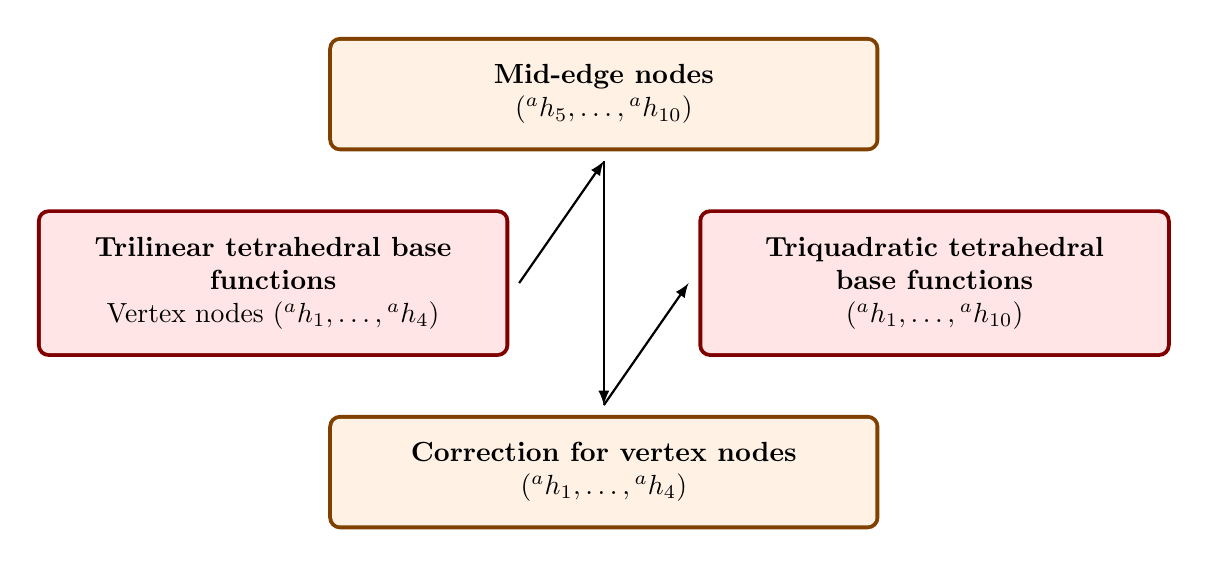
\begin{tikzpicture}[scale=0.6]
        \node (trilin) at (-2,0) {
            \begin{tcolorbox}[colframe=red!50!black, colback=red!10, coltitle=black, rounded corners, width=6cm]
                \centering \textbf{Trilinear tetrahedral base functions} \\ Vertex nodes $({}^ah_1,\dots,{}^ah_4)$
            \end{tcolorbox}
        };
        \node (edge) at (5,4) {
            \begin{tcolorbox}[colframe=orange!50!black, colback=orange!10, coltitle=black, rounded corners,width=7cm]
                \centering \textbf{Mid-edge nodes} \\ $({}^ah_5,\dots,{}^ah_{10})$
            \end{tcolorbox}
        };
        \node (corr) at (5,-4) {
            \begin{tcolorbox}[colframe=orange!50!black, colback=orange!10, coltitle=black, rounded corners,width=7cm]
                \centering \textbf{Correction for vertex nodes}  \\ $({}^ah_1,\dots,{}^ah_{4})$
            \end{tcolorbox}
        };
        \node (triquad) at (12,0) {
            \begin{tcolorbox}[colframe=red!50!black, colback=red!10, coltitle=black, rounded corners, width=6cm]
                \centering \textbf{Triquadratic tetrahedral base functions} \\ $({}^ah_1,\dots,{}^ah_{10})$
            \end{tcolorbox}
        };
        \draw[thick, -latex] (trilin.east) -- (edge.south);
        \draw[thick, -latex] (edge.south) -- (corr.north);
        \draw[thick, -latex] (corr.north) -- (triquad.west);
    \end{tikzpicture}
\end{frame}

\end{document}